\documentclass[11pt]{article}
\usepackage{graphicx} % Required for inserting images
\usepackage[top=2.5cm, bottom=2.5cm, left=2cm, right=2cm]{geometry}
\usepackage[T1]{fontenc}
\usepackage{wrapfig}
\usepackage{hyperref}
\usepackage[utf8]{inputenc}
\usepackage{multirow}
\usepackage{subcaption}
\usepackage{booktabs}
\usepackage{bookmark}
\usepackage{graphicx}
\usepackage{setspace}
\usepackage{listings}
\usepackage{xcolor}  % Opcional, per colors
\lstset{
  language=Python,
  basicstyle=\ttfamily\small,
  keywordstyle=\color{blue},
  commentstyle=\color{gray},
  stringstyle=\color{green!50!black},
  showstringspaces=false,
  numbers=left,
  numberstyle=\tiny\color{gray},
  frame=single,
  breaklines=true,
  captionpos=b,
  tabsize=4
}

\setlength{\parindent}{0in}
\usepackage{physics}
\usepackage{tikz}
\usepackage{tikz-3dplot}
\usepackage[outline]{contour} % glow around text
\usepackage{xcolor}
\usepackage{float}
\usepackage{makeidx}
\usepackage{fancyhdr}
\usepackage{pgfplots}
\usepackage{amsmath}
\pgfplotsset{compat=1.18}
\usepackage{caption}
\usepackage[english,catalan]{babel}
\setlength{\parskip}{11pt}
\usepackage{xcolor}
\usepackage{listings}
\usepackage{marginnote}
\usepackage{siunitx}
\usepackage{framed}
\usepackage{ulem}

\usepackage{titlesec}
\titleformat{\section}
  {\normalfont\Large\bfseries}
  {}
  {0pt}                
  {}  

\numberwithin{equation}{section}
\numberwithin{figure}{section}
\numberwithin{table}{section}

\begin{document}

\begin{titlepage}
    \centering
    \vspace*{\fill}

    {\Huge \bfseries Informes de Laboratori d'electromagnetisme\par}
    \vspace{2cm}
    
    {\Large \textbf{Grup A6}\par}
    \vspace{1cm}
    
    {\Large
    \begin{tabular}{c}
    Isaac Baldi García (1667260)\\
    Víctor Bosch González (1676373) \\
    Eira Jacas García (1666616) \\
    Miguel Ordejón de Prada (1710966)
    
    \end{tabular}
    }
    
    \vspace{1cm}

    {\large Maig de 2025\par}

    \vspace*{\fill}
\end{titlepage}

\tableofcontents
\newpage
\vspace{10em}
\section{\huge \textbf{Pràctica 1}}  % Títol petit en negreta

\vspace{0.5em}  % Espai vertical

{\Huge \textbf{Representació de camps}}  % Títol gran

\vspace{2em}  % Espai abans del contingut

%\title{\Huge\bfseries Pràctica 1 \\ Feixos de raigs catòdics \\ [2ex] \Large}

\begin{abstract}
    En aquesta pràctica estudiem el potencial i el camp elèctric en un medi dielèctric (lineal, isòtrop i homogeni) de tres distribucions de càrrega amb simetria translacional en l'eix vertical. Un condensador de plàques plano-paral·leles, dos fils infinits i una geometria escollida entre els membres del grup que replica la disposició d'un experiment de difracció. Per estudiar el camp elèctric aprofitem la simetria de les distribucions de càrrega que ens permet simplificar el nostre sistema de tres dimensions a dues dimensions. També aprofitem la dualitat entre el camp de desplaçament elèctric i el camp de densitat de corrent elèctric per determinar el potencial del camp elèctric mesurant el potencial del camp de corrents. Els resultats obtinguts són corroborats per simulacions computacionals i comparats amb els resultats del cas ideal dels què en difereix substancialment. També s'obté experimentalment la capacitat del condensador i es conclou que no difereix significativament del càlcul ideal.
\end{abstract}


\subsection{Introducció teòrica}\label{sec: intro}
En aquesta pràctica trobem experimentalment les línies equipotencials i de camp del camp elèctric de tres distribucions de càrrega en un material dielèctric (lineal, isòtrop i homogeni) de difícil o inexistent solució analítica, així com alguna propietat associada. La primera distribució estudiada és un condensador de plaques plano-paral·leles d'altura infinita i llargada finita, del qual també en calculem la capacitat; la segona són dos fils infinits paral·lels a diferents potencials; i per últim, estudiem una placa amb una escletxa davant d'un fil infinit, a diferents potencials.

Per estudiar aquestes distribucions de càrregues dins un medi dielèctric usem la dualitat que existeix entre el camp de corrents, $\vec{J}$, i el camp de desplaçament elèctric, $\vec{D}$. Com podem veure a les Eqs. (\ref{eq: J_D}) aquests dos camps tenen les mateixes equacions i, per tant, si repliquem les condicions de contorn d'un sistema en medi dielèctric en un sistema en medi conductor, obtindrem les mateixes solucions per les corrents que obtindrem en el sistema dielèctric pel camp de desplaçament.
\begin{equation}
    \begin{array}{lll}
    \vec{\nabla} \times \vec{J}=0 & \vec{J}=\sigma \vec{E} & \vec{\nabla} \cdot \vec{J}=0 \\
    \vec{\nabla} \times \vec{D}=0 & \vec{D}=\epsilon \vec{E} & \vec{\nabla} \cdot \vec{D}=0
    \end{array}
    \label{eq: J_D}
\end{equation}
Considerant que el medi dielèctric és lineal, isòtrop i homogeni (l.i.h), com veiem a les Eqs. (\ref{eq: J_D}), a través del camp de desplaçament i la permitivitat del medi dielèctric podem obtenir fàcilment la solució del camp elèctric i conseqüentment del potencial. A més, com que en aquest cas $\varepsilon$ i $g$ són escalars, el potencial complirà l'equació de Laplace a les regions amb càrrega lliure nul·la
\begin{equation}
    \div{\vec{D}}=\rho_F=0 \implies \div{(\varepsilon\vec{E})}=0\implies-\varepsilon\div{\div{\phi}}=0\implies\laplacian{\phi}=0.
\end{equation}
Així, usant un paper de carbó de conductivitat $g$ (que equival al medi dielèctric de permitivitat $\varepsilon$) i dibuixant-hi amb tinta conductora el sistema de càrrega podem fer mesures del potencial que generaran els corrents i relacionar-lo amb el potencial elèctric de la mateixa distribució de càrrega en un medi dielèctric.
Concretament, en aquesta pràctica els objectius que ens proposem són:
\begin{list}{$\ast$}{\leftmargin=1em}
    \item Determinar les línies equipotencials i de camp elèctric experimentals de
        \begin{enumerate}{\leftmargin=1em}
            \item  Un condensador de plaques plano-paral·leles d'alçada infinita però llargada finita.
            \item  Dos fils infinits paral·lels a diferents potencials.
            \item  Una placa amb una escletxa paral·lela a un fil infinit a diferents potencials.
        \end{enumerate}  
        i comparar-les amb els resultats simulats i els càlculs teòrics del cas ideal.
    \item Determinar la capacitat per unitat de longitud del condensador.
    \item Estudiar algun fenomen físic relacionat amb les línies equipotencials a través de la tercera configuració de càrrega, proposada pel grup.
\end{list}

Per assolir el primer objectiu, procedirem com s'explica a la Secció \ref{sec: metode}.

Pel que fa al càlcul experimental de la capacitat del condensador (segon objectiu), anomenant $l$ a la llargada de les plaques (cap a la direcció $Y$), $L$ una altura arbitrària (cap a la direcció $Z$) i $d$ la distància de separació entre les plaques, podem procedir de la següent manera.
A partir de dues línies equipotencials que tanquin una de les plaques del condensador podem calcular la càrrega per unitat de longitud.
\begin{equation}
    \frac{Q}{L} = \frac{1}{L}\oint\vec{D}\vec{ds}=\varepsilon\oint Edl\approx \varepsilon \sum_i E_i \, \Delta l_i \approx \varepsilon \sum_i \frac{\Delta \phi_i \, \Delta l_i}{\Delta r_i}
    \label{eq: Q}
\end{equation}
On $\frac{Q }{L }$ és la càrrega per unitat de longitud del condensador, $\varepsilon$ la peritivitat del medi dielèctric, $\Delta \phi_i$ la diferència de potencial entre les línies equipotencials, $\Delta l_i$ un petit increment de distància sobre la línia equipotencial interior i $\Delta r_i$ la distància en aquest punt entre la línia equipotencial interior i l'exterior.
Aleshores, podem calcular la capacitat per unitat de longitud si sabem el potencial aplicat entre les plaques, $\Delta V$.
\begin{equation}
    \frac{C}{L}=\frac{Q/L}{\Delta V}
    \label{eq: C}
\end{equation}

Per altra banda, per obtenir la capacitat ideal d'un condensador de plaques plano-paral·leles com el que tenim a l'experiment calculem la diferència de potencial entre les plaques,
\begin{equation}
    |\Delta\phi|=\int_{0}^{d} \vec{E}\vec{dl}= Ed,
\end{equation}
i com que assumim que el camp és uniforme i de valor $\frac{\sigma}{\varepsilon}$\footnote{És molt fàcil obtenir aquest resultat sumant el camp de dos plans infinits de càrrega oposada que s'obté amb la llei de Gauss} podem obtenir la capacitat per unitat de longitud de la següent manera:
\begin{equation}
    \Delta\phi=Ed=\frac{\sigma d}{\varepsilon}
    =Q\frac{d}{lL\varepsilon}=\frac{Q}{C}\implies (\frac{C}{L})_t=\frac{l}{d}\varepsilon
    \label{eq: c_t}
\end{equation}

En relació a l'últim objectiu, la tercera configuració estudiada és un fil infinit enfront d'una placa infinita en l'eix $Z$ amb una escletxa al llarg de la placa i al davant del fil. A més, existeix una diferència de potencial entre el fil i les dues parts de la placa, què sí que estan al mateix potencial. Aquesta és una disposició similar a la d'un experiment de difracció si tractem el fil com un "emissor" de línies equipotencials i les plaques amb l'escletxa com l'objecte que les difracta. Per tant, la motivació per estudiar aquesta configuració prové de voler veure si amb les línies de potencial passa algun fenomen similar a la difracció d'ones\footnote{Més informació sobre la difració d'ones a \url{https://en.wikipedia.org/wiki/Diffraction}}.

\subsection{Mètode experimental}\label{sec: metode}
Per dur a terme l'experiment hem dibuixat les tres configuracions esmentades anteriorment sobre uns rectangles de paper de carbó (de $28cm\cross20cm$) amb tinta conductora de plata. Així doncs, hem traduït els nostres sistemes de tres dimensions (però amb simetria translacional en un eix) a sistemes de dues dimensions dibuixant sobre el paper la secció de les geometries cap a la direcció $Z$. Per exemple, el condensador s'ha convertit en dues línies paral·leles i els dos fils infinits en dos punts. A l'Annex \ref{fotos} hi ha imatges de les tres configuracions que hem muntat al laboratori. Tot seguit, quan la tinta era seca (s'ha d'esperar uns 20 min), hem connectat el sistema a una font de corrent amb una diferència de potencial de $15 V$. En aquest moment és molt important comprovar que el conductor està ben dibuixat mirant si tots els punts de l'elèctrode tenen el mateix potencial. Finalment, amb un voltímetre hem anat marcant punts amb el mateix potencial per poder dibuixar les línies equipotencials.

En el cas del condensador és important que tingui les dimensions adequades. Ha de ser prou petit per obtenir línies tancades i que $\frac{d}{l}$ sigui prou petit perquè aquestes siguin paral·leles a la zona central del condensador. Unes bones mides per la dimensió del nostre paper són: $d=3cm$ i $l=8cm$.
Pel que fa al sistema de fils infinits, que sobre el paper representem com dos punts, és important que aquests siguin prou grans perquè les forquilles amb què els connectem a la font de corrent hi càpiguen i no generin interferències.

Per obtenir les dades necessàries pel càlcul de la capacitat del condensador, primerament hem dibuixat dues línies equipotencials tancades al voltant d'una de les plaques. Després hem dividit la línia interna en 20 segments i hem anat mesurant la llargada de cada segment ($\Delta l_i$), conjuntament amb la distància del segment a la línia equipotencial externa ($\Delta r_i$) i la diferència de potencial entre les dues línies ($\Delta \phi_i$).

Per representar els punts experimentals els hem digitalitzat amb el programa web WebPlotDigitizer\copyright\footnote{Enllaç a l'aplicació web: \url{https://automeris.io/wpd/}}. Així, també hem pogut dibuixar el camp elèctric calculant la direcció perpendicular a la recta entre dos punts experimentals adjacents amb un programa de Python.

Finalment, hem fet una simulació en Python per calcular computacionalment les línies equipotencials i de camp de les tres configuracions de conductors. Com veurem a la següent secció, la simulació no és del tot fidel amb la realitat. Per millorar-ne els resultats es pot mesurar el potencial a les vores del paper conductor i aplicar aquests valors com a condició de contorn a la simulació.\footnote{\label{nota: codis}Tots els codis es troben a l'Annex \ref{sec: python}}

\subsection{Resultats i discussió}\label{sec: resultats}
En aquesta secció presentem i comparem els resultats obtinguts tant experimentalment com computacionalment. Mostrem les línies de camp i les línies equipotencials de les tres distribucions de càrrega, així com el resultat experimental de la capacitat d'una d'elles. Per fer les simulacions hem solucionat l'equació de Laplace amb el mètode numèric de Jacobi\footnotemark[3]. Cal destacar que les simulacions les hem fet al buit, ja que no coneixem el valor de la permetivitat del dielèctric. A més, s'ha considerat que els elèctrodes són conductors ideals i constitueixen les úniques fonts del camp.

\subsubsection{Condensador de plaques plano-paral·leles}\label{sec: cond}
La primera distribució de càrrega que estudiarem és un condensador de plaques plano-paral·leles centrat a l'origen. Les plaques són paral·leles al pla $YZ$, finites en la direcció $Y$ i molt llargues o infinites en la direcció $Z$.
En les Figs. (\ref{fig: cond_pot}) i (\ref{fig: cond_e}) podem veure representades les línies de camp elèctric i les línies equipotencials obtingudes tant experimentalment com en la simulació.   
\begin{figure}[h]
    \centering
    \begin{subfigure}{0.495\textwidth}
        \centering
        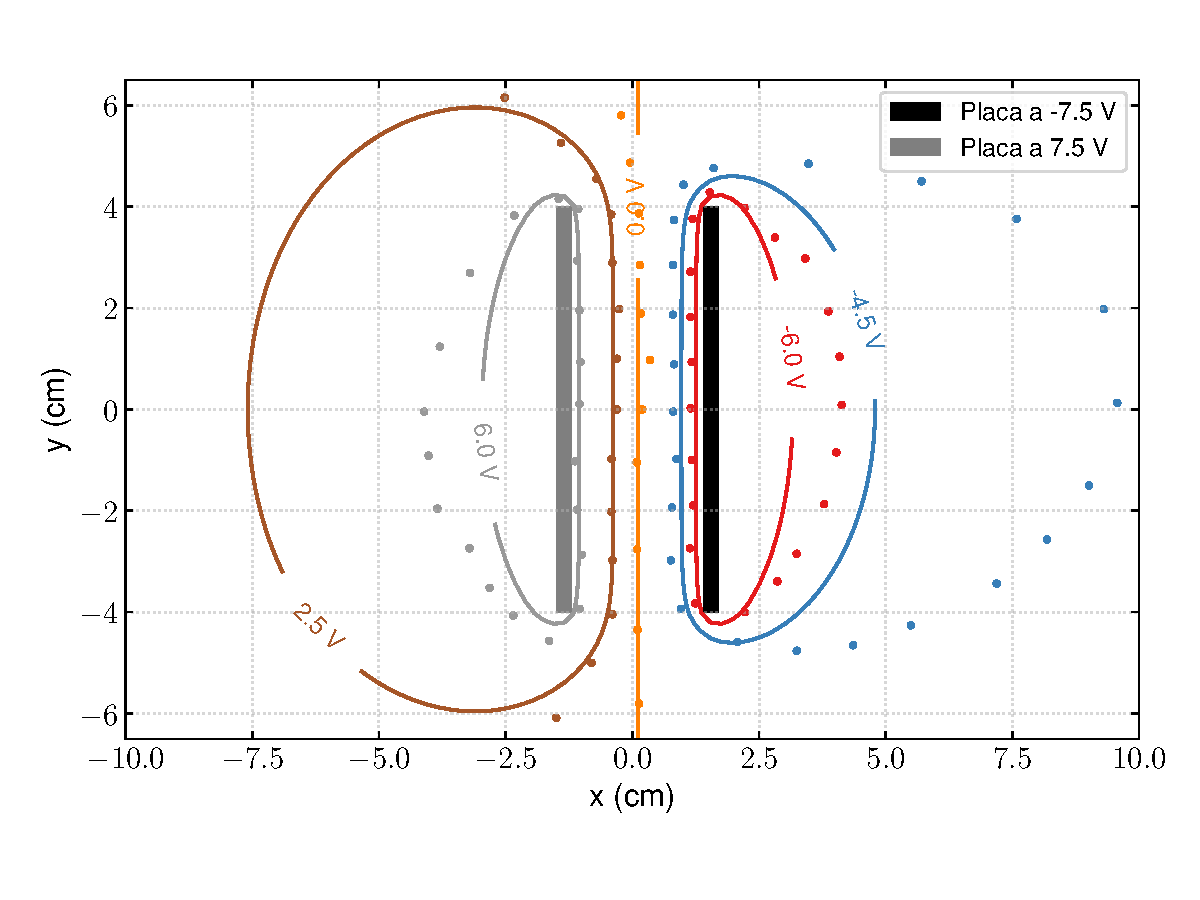
\includegraphics[width=\textwidth]{cond_combi_def.pdf}
        \caption{Línies equipotencials d'un condensador plano-paral·lel. Punts experimentals i línies de la simulació.}
        \label{fig: cond_pot}
    \end{subfigure}
    \begin{subfigure}{0.495\textwidth} 
        \centering
        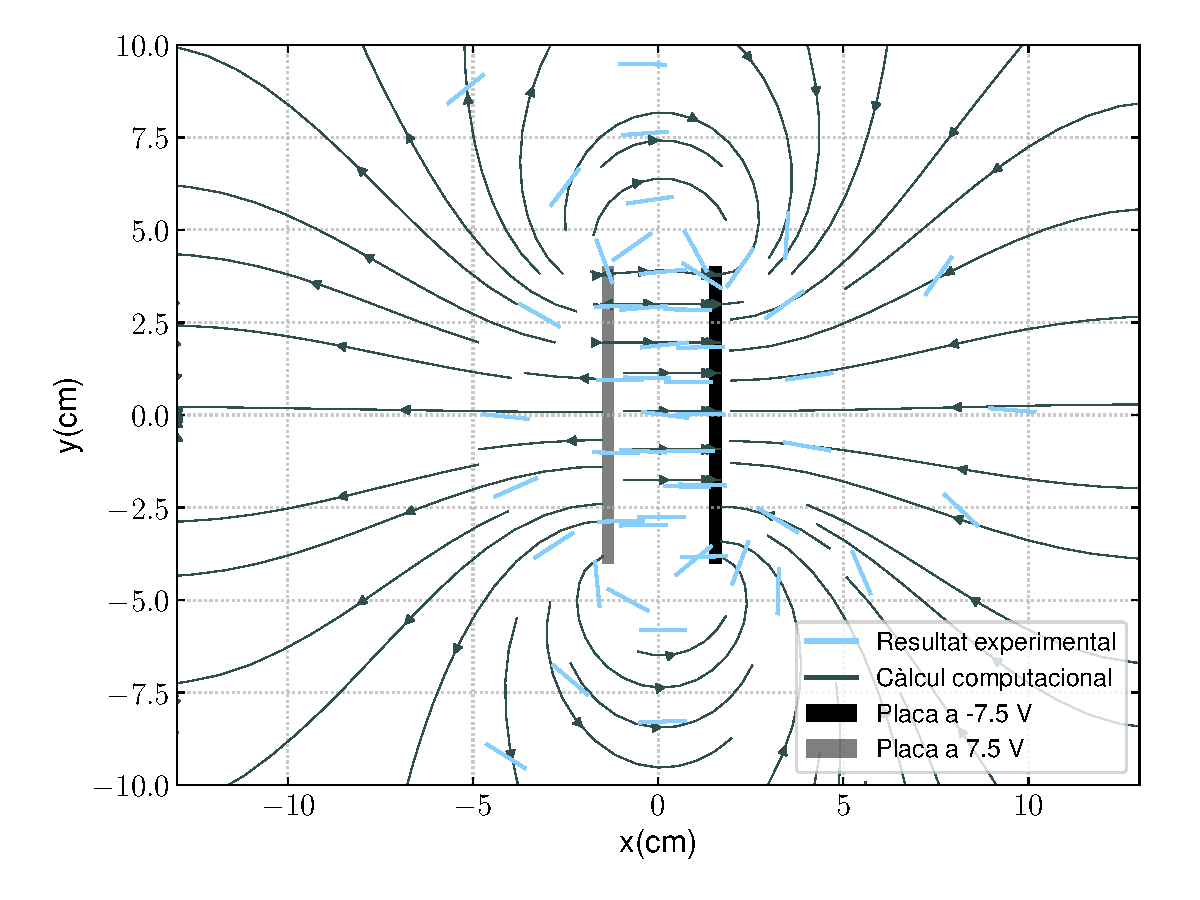
\includegraphics[width=\textwidth]{cond_camp.pdf}
        \caption{Línies de camp elèctric d'un condensador plano-paral·lel. Segments experimentals i línies de la simulació.}
        \label{fig: cond_e}
    \end{subfigure}
\end{figure}

A la Fig. (\ref{fig: cond_pot}) s'observa com a la regió central del condensador les línies equipotencials són paral·leles a les plaques, com prediu la teoria. En canvi, a prop de les vores, les línies es corben fins que s'acaben tancant. La disminució de la component $Y$ del camp elèctric provoca aquesta corbatura i es deu a que en aquesta direcció ens allunyem de la placa, és a dir, de la font de camp. Aquest resultat difereix del cas ideal (condensador de plaques infinites), en el qual les línies equipotencials mai es tanquen. Tanmateix, veiem que coincideix amb la simulació, on les línies també es tanquen tot i que ho fan més a prop. Aquesta discrepància entre la simulació i l'experiment principalment és a causa de que a la simulació no hem introduït la condició de contorn relacionada amb els límits del paper conductor. També hi ha altres efectes com les irregularitats dels elèctrodes, la connexió entre la font i els elèctrodes o les possibles fluctuacions de la idealitat del medi que no hem tingut en compte a la simulació i poden contribuir a la diferència dels resultats.

Pel que fa a la Fig. (\ref{fig: cond_e}) veiem com les línies de camp van des de la placa positiva a la negativa (com era d'esperar) i tenen major densitat a prop d'aquestes, indicant que el camp és més intens. Com en el cas del potencial, les línies segueixen un comportament semblant al ideal a la part central i, en canvi, a prop de les vores es desvien a causa dels efectes de vorada. Similarment, els segments experimentals, que representen la direcció del camp, també segueixen la tendència del càlcul computacional tot i que les línies experimentals tendeixen a tancar-se més sobre els elèctrodes. Aquestes diferències s'expliquen igual que les discutides anteriorment.

Per calcular la capacitat del condensador, primer hem calculat la càrrega per unitat de superfície del condensador en funció de $\varepsilon$, a partir de l'Eq. (\ref{eq: Q}). Tot seguit, amb l'Eq (\ref{eq: C}) hem calculat la capacitat per unitat de longitud del condensador (les dades necessàries per fer els càlculs es poden trobar a la Taula \ref{tab:mesures} de l'annex com també les Eqs. (\ref{eq: ins_q}), (\ref{eq: ins_c}) i (\ref{eq: ins_ct}) pel càlcul d'incerteses).

\[
\frac{Q}{L} = \varepsilon  (37{,}65 \pm 9{,}48)\, \mathrm{C/m} \implies
\boxed{ \frac{C}{L} = \varepsilon  (2{,}51 \pm 0{,}63)\, \mathrm{F/m} }
\]    

Aquest resultat el podem comparar amb el resultat teòric de la capacitat d'un condensador ideal amb les mateixes dimensions. Usant l'Eq. (\ref{eq: c_t}) obtenim $(\frac{C}{L})_t =\varepsilon(2,667 \pm 0,095)\, \mathrm{F/m}$ que és compatible amb el resultat experimental del nostre condensador no ideal.

\subsubsection{Fils infinits}\label{sec: fils}
La segona configuració estudiada són dos fils infinits paral·lels amb càrrega oposada. Conseqüentment, en aquest cas, la simulació representa el cas ideal.
\begin{figure}[h]
    \centering
    \begin{subfigure}{0.495\textwidth}
        \centering
        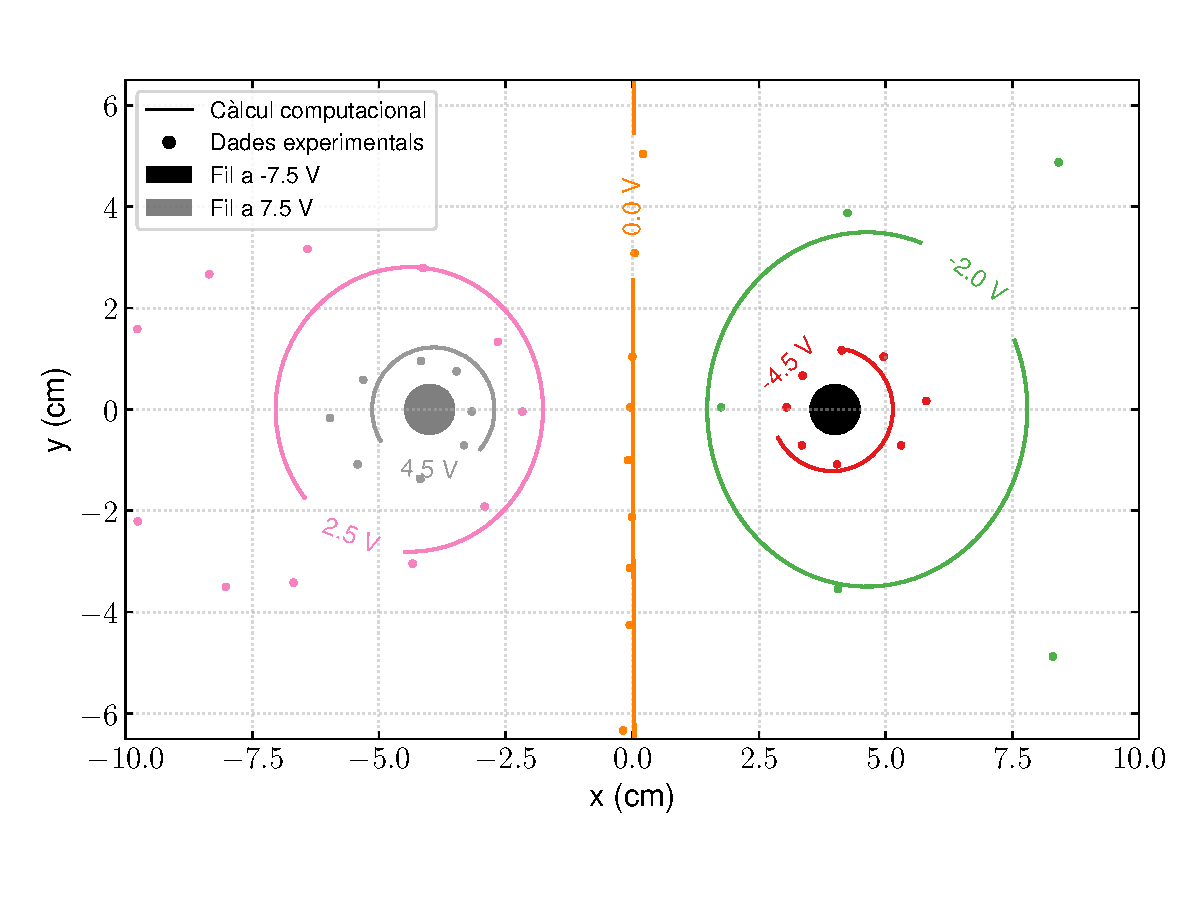
\includegraphics[width=\textwidth]{fils_combi.pdf}
        \caption{Línies equipotencials de dos fils infinits paral·lels i a potencials oposats.}
        \label{fig: fils_pot}
    \end{subfigure}
    \begin{subfigure}{0.495\textwidth} 
        \centering
        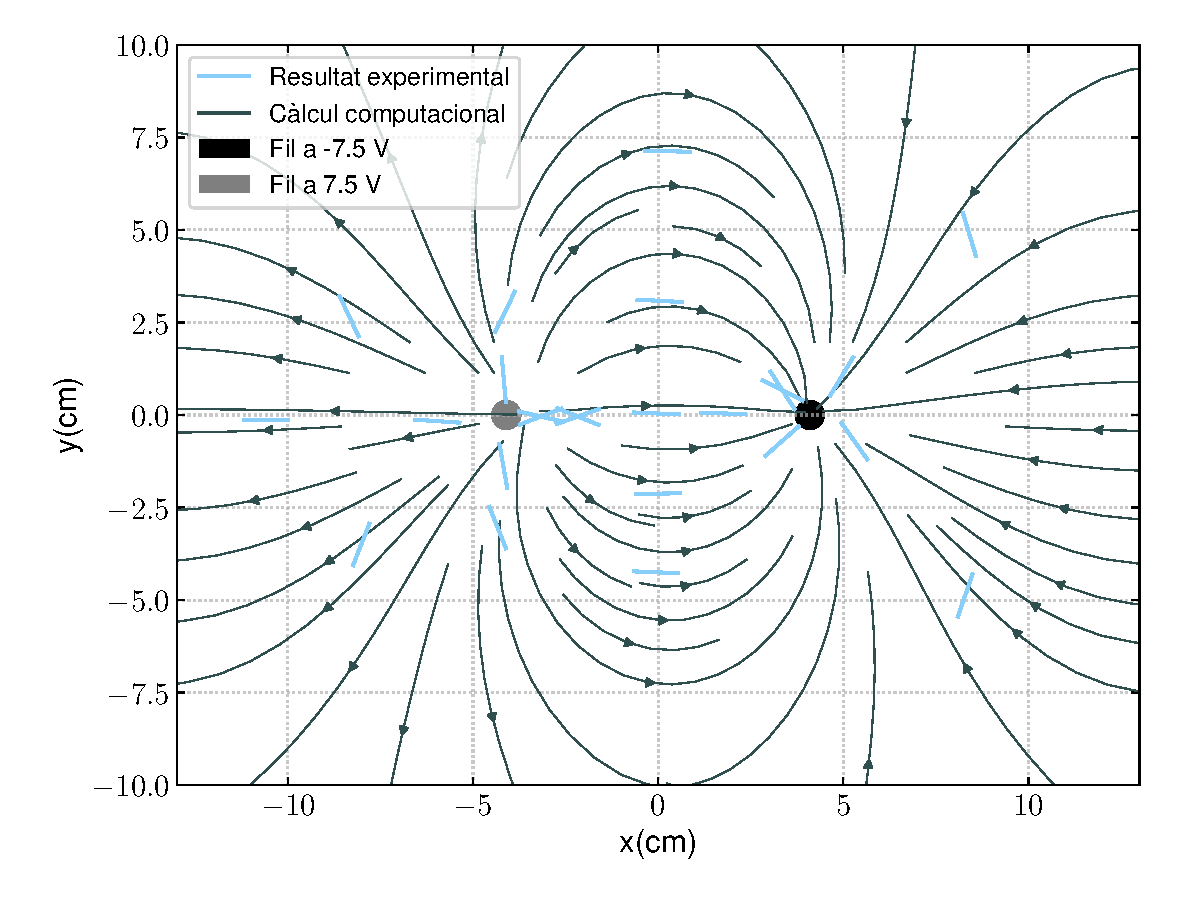
\includegraphics[width=\textwidth]{fils_camp.pdf}
        \caption{Línies de camp elèctric de dos fils infinits paral·lels i a potencials oposats. Segments experimentals i línies de la simulació.}
        \label{fig: fils_camp}
    \end{subfigure}
\end{figure}


A la Fig. (\ref{fig: fils_pot}), si ens fixem en les línies equipotencials experimentals veiem que es tanquen en el·lipses al voltant dels fils i presenten una línia vertical just entre els dos elèctrodes. Aquesta és la tendència dictada per la simulació tot i que en la simulació les línies es tanquen en circumferències. Aquesta diferència pot ser deguda a diversos factors. En primer lloc, el nostre sistema té una discontinuïtat en el medi als límits del paper (rectangular) que no hem introduït a la simulació i, al no tenir la mateixa geometria que el sistema, afecta la forma de les línies equipotencials. En segon lloc, el nostre muntatge experimental és una aproximació en dues dimensions del sistema en tres dimensions que intentem replicar. Per últim, pot haver altres contribucions al camp que no hem tingut en compte com la unió entre els elèctrodes i la font de corrent o un camp extern present al laboratori.

Per altra banda, el camp elèctric  experimental mostrat a la Fig. (\ref{fig: fils_camp}) també segueix la tendència de la simulació tot i que les línies de camp que surten del fil a $7.5$ V tenen més tendència a tancar-se cap al fil a $-7.5$ V. Això pot ser degut a que hi ha diversos efectes que no hem tingut en compte a la simulació com hem explicat en el cas del potencial. 

\subsubsection{Placa amb escletxa i fil infinit}\label{sec:lliure}
La tercera configuració estudiada és un fil infinit enfront una placa infinita en l'eix $Z$ amb una escletxa al llarg de la placa i al davant del fil. A més, existeix una diferència de potencial entre el fil i les dues parts de la placa, què sí que estan al mateix potencial. Aquesta, és una disposició similar a la d'un experiment de difracció si tractem el fil com un "emissor" de línies equipotencials i les plaques amb l'escletxa com l'objecte que les difracta.

\begin{figure}[h]
    \centering
    \begin{subfigure}{0.495\textwidth}
        \centering
        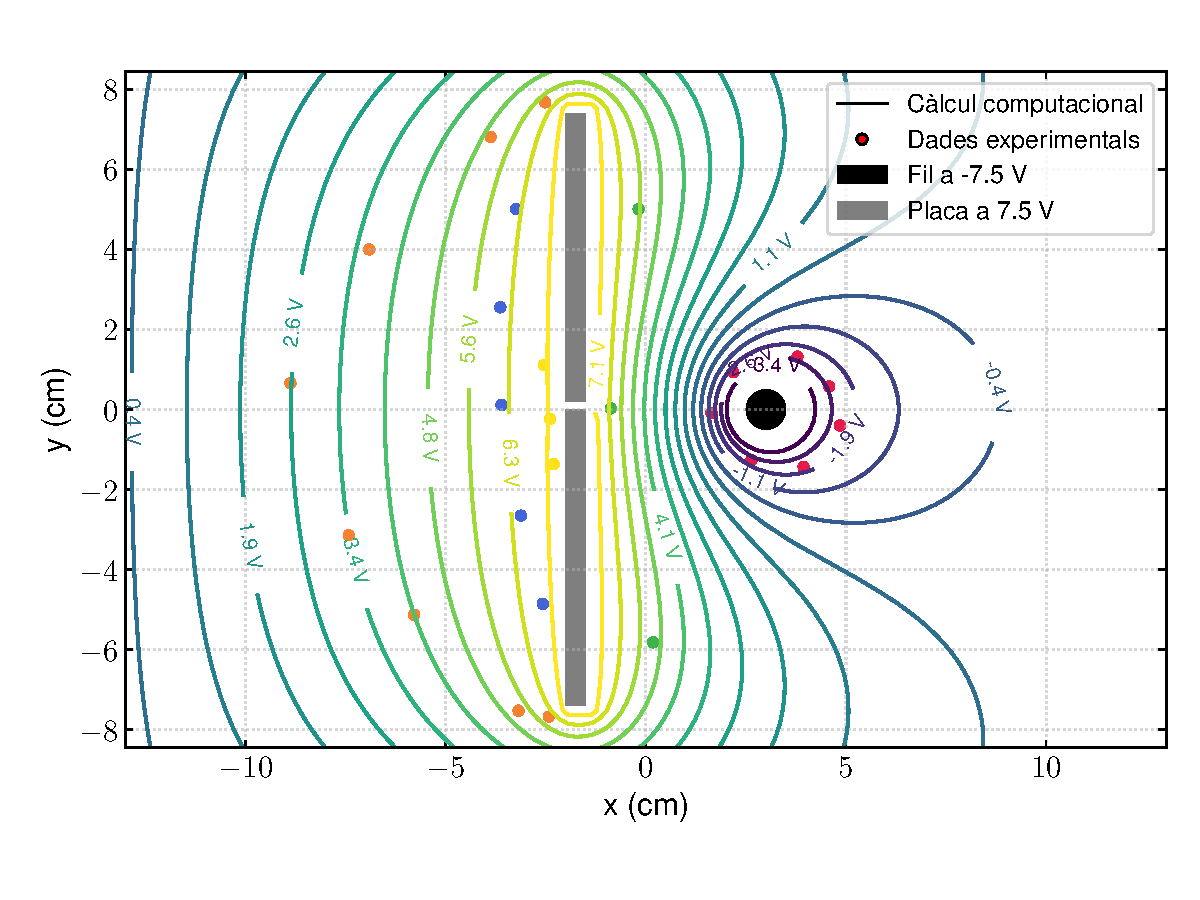
\includegraphics[width=\textwidth]{lliure_combi_e_colors.pdf}
        \caption{Línies equipotencials d'una placa infinita AMB escletxa davant d'un fil infinit. Punts experimentals de color diferent per cada valor de potencial.}
        \label{fig: lliure_pot_e}
    \end{subfigure}
    \begin{subfigure}{0.495\textwidth} 
        \centering
        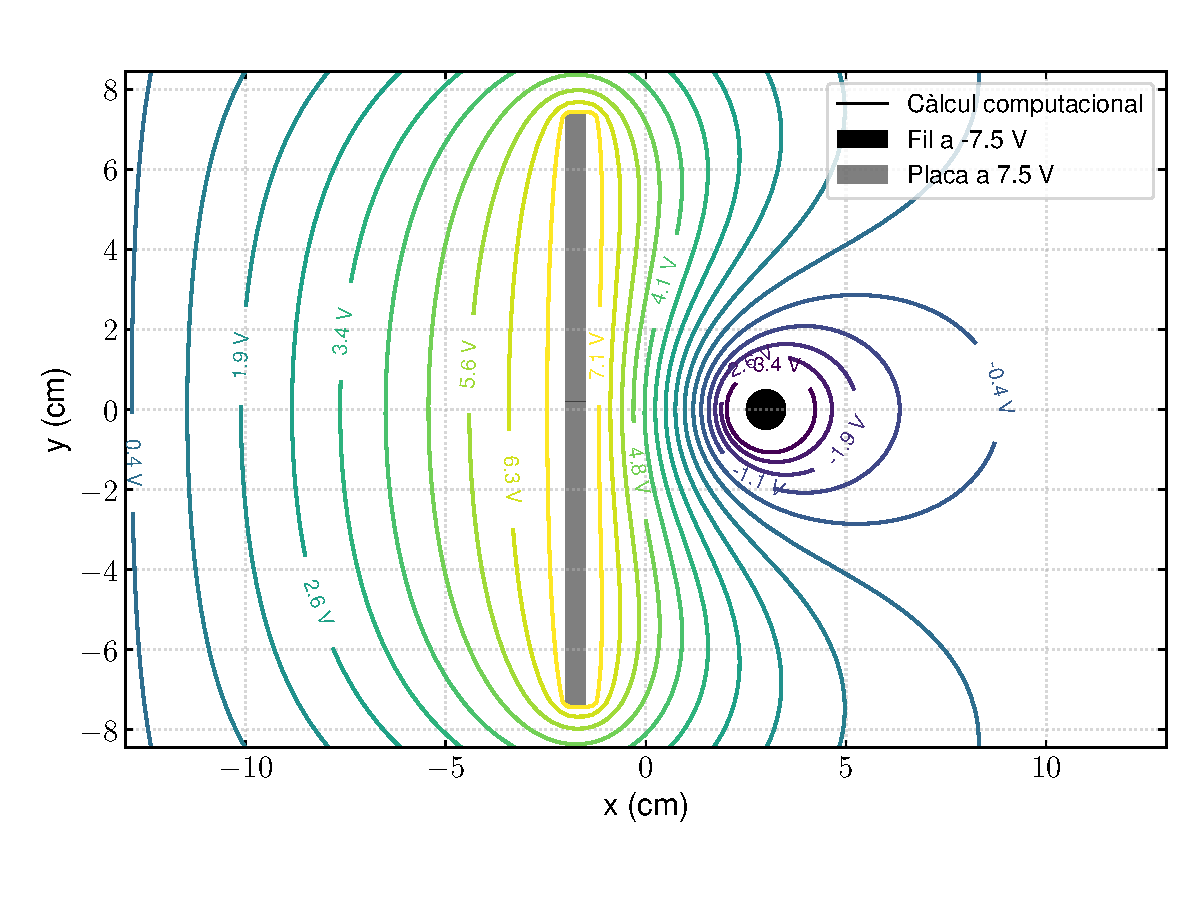
\includegraphics[width=\textwidth]{lliure_combi_0.pdf}
        \caption{Línies equipotencials d'una placa infinita SENSE escletxa davant d'un fil infinit.}
        \label{fig: lliure_pot_0}
    \end{subfigure}
\end{figure}
Si ens fixem en les línies equipotencials experimentals de la Fig. (\ref{fig: lliure_pot_e}) veiem que es comporten de la següent manera: el radi de corvatura de les línies equipotencials va augmentant a mesura que ens allunyem de l'"emissor" (fil) i ens apropem a l'escletxa, tal com ho faria el front d'una ona. A l'altra banda de l'escletxa, el radi de corvatura disminueix respecte l'observat abans de l'escletxa de tal forma que és com si l'escletxa fos un segon emissor. Per tant, amb aquesta informació sembla que hi hagi hagut un fenòmen de difracció degut a l'escletxa.
No obstant això, si ens fixem en les línies equipotencials simulades veiem clarament que el motiu de la forma de les línies equipotencials no té res a veure amb l'escletxa. El veritable fet que explica les línies equipotencials mostrades és la superposició del potencial elèctric generat pel fil i la placa (que ja en coneixem la forma gràcies a les configuracions anteriors). De fet, com podem veure a la Fig. (\ref{fig: lliure_pot_0}) l'existència de l'escletxa quasi bé no afecta a la forma de les línies equipotencials, ja que és molt petita en comparació amb les dimencions del fil i de la placa. Per tant, la difracció no serveix per explicar les observacions experimentals, tot i que, experimentalment, en un principi ho pugui semblar. Aquest resultat, era d'esperar ja que el potencial d'un sistema electroestàtic, per començar, no depen del temps i, per tant, no pot tenir propietats ondulatòries.
\begin{figure}
    \centering
    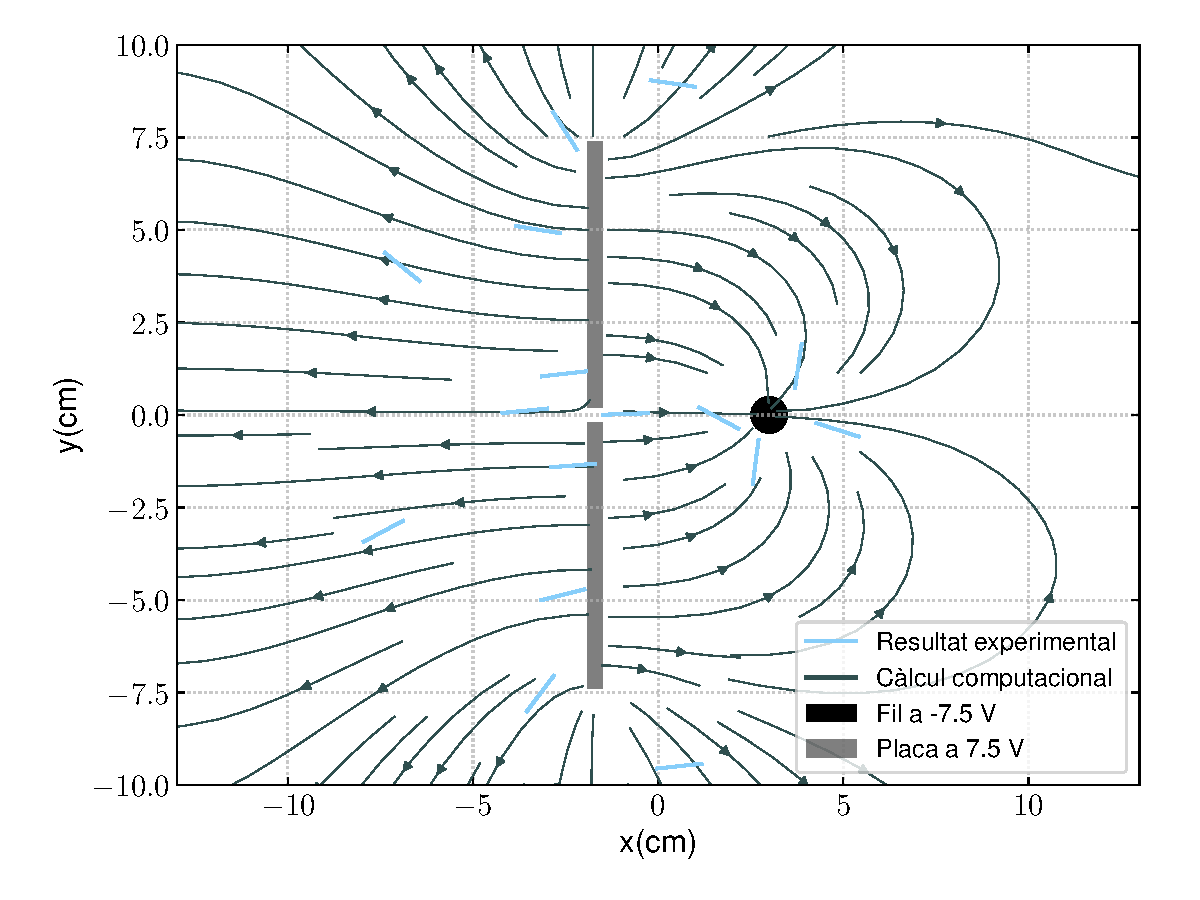
\includegraphics[width=0.45\textwidth]{lliure_camp.pdf}
    \caption{Línies de camp elèctric. Segments experimentals i línies de la simulació.}
    \label{fig: lliure_camp}
\end{figure}

Per altra banda, a la Fig. (\ref{fig: lliure_camp}) podem veure el camp elèctric generat per aquesta configuració. Com en les altres configuracions veiem que el camp experimental segueixi la tendència de la simulació però es tanca més al voltant de les vores de les plaques i dels fils infinits. Aquestes diferències s'expliquen pels mateixos raonaments que en els casos anteriors.


\subsection{Conclusions}\label{sec: conc}

En aquesta pràctica hem estudiat les línies equipotencials i de camp dins d'un material dielèctric de tres configuracions de conductors diferents, gràcies al paral·lelisme entre les equacions del camp de corrents i del camp de desplaçament. 

En primer lloc hem estudiat un condensador de plaques plano-paral·leles finites només en una dimensió i hem pogut veure com, a diferència del cas ideal, les línies de camp es tanquen al voltant de les plaques. També hem vist com la simulació al buit coincideix en tendència amb l'experiment però les línies equipotencials simulades es tanquen més a prop de les plaques a causa que el camp elèctric al buit és més intens que en el dielèctric. A més, hem realitzat un càlcul experimental de la capacitat del condensador i hem obtingut un valor de $ \frac{C}{L} = \varepsilon  (2{,}51 \pm 0{,}63)\, \mathrm{F/m} $ que és compatible amb el resultat del model ideal.

En segon lloc hem estudiat dos fils infinits paral·lels a potencials oposats. En aquest cas hem pogut observar com les limitacions del nostre experiment per reproduïr aquesta configuració han provocat que les línies equipotencials fossin el·líptiques en comptes de circulars.

Per últim, hem estudiat una placa amb una escletxa davant d'un fil infinit a un potencial diferent amb l'objectiu de veure si les línies equipotencials pateixen algun fenomen similar a la difracció d'una ona a causa de l'escletxa. Tanmateix, amb l'experiment hem constatat que, no obstant les línies experimentals semblaven patir quelcom semblant a la difracció, amb la simulació hem pogut comprovar que la forma de les línies equipotencials quasi no depenia de si hi havia escletxa o no, i per tant, hem descartat aquesta idea.

\newpage
\section{\huge \textbf{Pràctica 2}}

{}  % Títol petit en negreta

\vspace{0.5em}  % Espai vertical

{\Huge \textbf{Força entre corrents}}  % Títol gran

\vspace{1em}  % Espai abans del contingut

\begin{abstract}
    En aquesta pràctica estudiem la força magnètica entre dos fils amb corrent elèctric de mateixa intensitat, en concret, analitzem la seva relació amb la magnitud de la intensitat dels fils i la dependència amb la distància que els separa. També s'aprofita el muntatge experimental per mesurar la component horitzontal del camp magnètic terrestre. Les dades experimentals es tracten mitjançant el mètode dels mínims quadrats per obtenir paràmetres que es poden comparar amb valors teòrics, en concret calcularem el valor de la permeabilitat magnètica al buit. Aquests presenten diferències prou significatives respecte als nostres resultats, el que creiem que és degut a la gran complexitat del mètode experimental emprat.
\end{abstract}

\subsection{Introducció}\label{sec: PR2_intro}

En aquesta pràctica tenim per objectiu estudiar la força magnètica que es genera entre dos fils paral·lels pels quals es fa passar corrent elèctric. També, aprofitarem el muntatge experimental per a mesurar la component normal del camp magnètic terrestre.

La força magnètica entre dos fils finits de corrent es calcula a través de la llei de Biot-Savart. Però tenint que la separació entre els fils de corrent és molt menor a la longitud d'aquests, podem arribar a considerar que el camp magnètic que rep un dels fils és el generat per un altre fil infinit situat paral·lelament a una certa distància d'ell. 

Aquesta aproximació ens facilita molt més els càlculs ja que podem trobar el camp magnètic generat per un fil infinit amb la llei d'Ampère, que ens dona com a resultat la següent expressió:

\begin{equation}\label{eq_PR2: PR2_camp_fil_infinit}
    B = \frac{\mu_0I}{2\pi r}
\end{equation}

I que la força magnètica que rep el fil d'una longitud $L$ és

\begin{equation}\label{eq: PR2_Fmagn_en_funcio_B}
    \vec{F} = I\int d\vec{l}\times\vec{B}(\vec{r})
\end{equation}

La força magnètica (el mòdul) resultant té l'expressió següent:

\begin{equation}\label{eq: PR2_Fm_entre_fils}
    F = \frac{\mu_0I^2L}{2\pi r}
\end{equation}

Per mesurar la força magnètica entre dos fils de corrent i la seva dependència amb la intensitat de corrent que hi circula i amb la distància de separació entre ells utilitzarem una balança. Aquesta permet saber quan el sistema està en equilibri, és a dir, quan la força magnètica generada pels fils és compensada per una altra força d'igual direcció però de sentit contrari. 

Aquesta altra força, que ha de ser fàcilment parametritzable, pot correspondre a la força de la gravetat associada al fil superior. La qual mesurarem a través de les masses conegudes que col·locarem sobre la cassoleta que té aquest fil.

També pot correspondre a la força de torsió del sistema que conté el fil superior. La qual es pot mesurar a través de l'angle de gir resultant del fil superior al rebre la força magnètica.
 
La força de la gravetat segueix la següent equació

\begin{equation}\label{eq: PR2_Fgrav}
    F_{grav} = mg
\end{equation}

On $m$ correspon a la massa coneguda col·locada sobre la cassoleta i $g$ és la gravetat de la terra, la qual agafem com a constant amb valor $g = 9,81 \, m/s^2$\footnote{Valor mitjà tabulat extret de la Viquipèdia}

I la força de torsió

\begin{equation}\label{PR2_Ftorsio}
    F_{tor} = k\theta
\end{equation}

On $k$ és la constant de torsió del fil superior i $theta$ l'angle de torsió del fil, prenent com a 0º la posició que té el fil superior quan no rep força de l'altre fil.

\subsection{Mètode Experimental}\label{sec: PR2_met_exp}

La balança de corrent està formada per un marc rectangular per on hi circula un corrent. Aquest es troba sustentat pel fil de torsió i es troba sotmès a un equilibri entre la força del contrapès i la força entre fils. 

Per tal d'afavorir el moviment del rectangle conductor, les connexions entre el marc i la font de corrent es fan usant gal·li líquid. Els motius pels quals s'usa el gal·li són la seva baixa temperatura de fusió (29ºC) i el seu preu econòmic. El metall fos permet la mobilitat del marc i proporciona una connexió contínua i gairebé sense presentar fricció. S'obren els pots de gal·li i es connecta el transformador de corrent de $9 V$ per fondre'l. 

A continuació, es posen en contacte els pots de gal·li amb el marc rectangular, que té unes petites puntes sobresortint que entren perfectament en l'obertura de cada pot de gal·li. També es connecta el transformador amb el fil inferior per que aquest també tingui corrent circulant-hi.

%DIBUIX MUNTATGE

\begin{figure}[H]
    \centering
    \begin{subfigure}{0.4\textwidth}
        \centering
        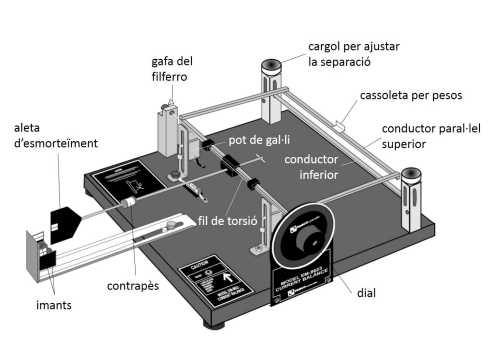
\includegraphics[width=0.5\textwidth]{PR2_dib_muntatge_parts.jpg}
        \caption{Parts de la balança usada en l'experiment.}
        \label{fig: PR2_dib_muntatge_parts}
    \end{subfigure}
    \hspace{0.1\textwidth}
    \begin{subfigure}{0.4\textwidth}
        \centering
        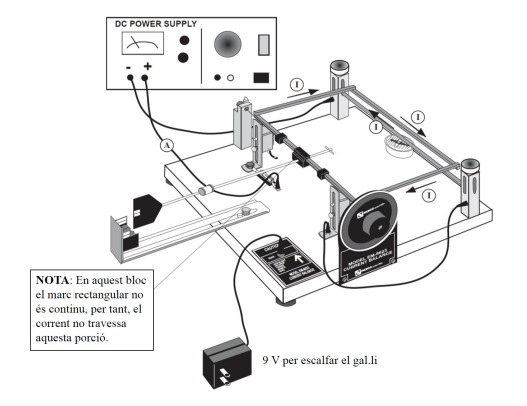
\includegraphics[width=0.5\textwidth]{PR2_dib_muntatge_corrent.jpg}
        \caption{Connexions per a fer circular corrent pels fils de la balança.}
        \label{fig: PR2_dib_muntatge_corrent}
    \end{subfigure}
\caption{Muntatge de la balança usada}
\end{figure}

La importància de la presa de mesures en aquesta pràctica recau en la calibració de la balança. Primerament, es col·loca la balança de tal forma que els cables siguin paral·lels al camp magnètic terrestre, seguint la direcció que ens indica la brúixola. Així, es pot eliminar la contribució del camp
magnètic terrestre, que alteraria els resultats. 

En segon lloc ajustem les potes de les potes de tal manera que la bombolla quedi al centre de l'espai disponible que te per moure's, fet que indica que està completament paral·lela al pla z. A continuació, ens assegurem que el dial de torsió del marc rectangular està al zero. 

Finalment, es mou el contrapès fins que la balança estigui estable i després es mou el cursor de marques, que conté uns imants per disminuir l'oscil·lació de l'aleta d'amortiment fins que ens quedin alineades amb la marca de l'aleta.

Després de fer una mesura, la balança pot quedar descalibrada (l'aleta d'amortiment no queda alineada amb el cursor de marques). Si aquest és el cas, cal tornar a calibrar la balança de nou.

Un cop la balança calibrada, la pràctica es divideix en 3 parts. En la primera part, es fan girar els cargols 5 voltes completes de tal forma que se separen els cables 5 mm més. A continuació es posa la massa de 5 mg i es connecta la font de corrent continu augmentant la intensitat fins que
s'equilibra la balança. Es repetirà el mateix procés per a les diferents masses, augmentant-les de 5 mg en 5 mg a cada nova mesura.

En la segona part de la pràctica, es posa la massa de $5 \, mg$ sobre la cassoleta i es gira el dial ens que la balança torni a l'equilibri. Seguidament es repeteix el procés per les masses de 10, 15, 20 i 25 mg i a continuació es van separant els fils a I constant (girant les rodetes que desplacen el fil inferior) per a trobar el valor de $\mu_o$.

Finalment, en la tercera part de la pràctica es rota el sistema 90 graus de manera que sigui el camp de la Terra qui faci la força sobre el fil de corrent (recordem que fins ara el teníem paral·lel al camp de la Terra perquè aquest no fes cap força sobre el fil). A continuació, es desconnecta la intesitat del cable inferior i pel superior es fa circular la major intensitat possible. Finalment, es gira el dial fins a equilibrar la balança. D’aquesta manera, mesurant la força que rep el fil es podrà trobar de quina magnitud és el camp causant d’aquesta força.

Per a una intensitat determinada, la força que rep el fil ve donada per l’Eq. \eqref{eq: PR2_Fmagn_en_funcio_B}, i simplement aïllant el camp es podria trobar el seu valor:

\begin{equation}\label{eq: PR2_Btnorm}
    B_{t_{norm}} = \frac{k\theta}{LI}
\end{equation}

On $k$ representa la constant de torsió trobada en la segona part de la pràctica, $\theta$ els graus necessaris per equilibrar la balança, $L$ la longitud del fil de corrent i $I$ la intensitat d'aquest.

%EQUILIBRAT DE LA BALANÇA

Per saber si el sistema es troba en equilibri cal fixar-nos en que les 3 línies, les dues del cursor de marques i la de l'aleta d'amortiment es trobin perfectament alineades. 

\iffalse
DIBUIX LLENGUETES
\begin{figure}[H]
    \centering
    \includegraphics[width=0.5\textwidth]{PR2_dib_llenguetes.jpg}
    \caption{Posició de les llenguetes quan balança està en equilibri.}
    \label{fig: PR2_dib_llenguetes}
\end{figure}
\fi

A la pràctica, l'aleta d'amortiment mai es quedava en una posició sense moviment. Així doncs, preniem com sistema en equilibri vàlid per a la mesura quan l'aleta patia la mínima osicil·lació possible, d'amplitud constant (igual desplaçament amunt i avall).

\subsection{Presentació i discussió de resultats}\label{sec: PR2_resultats}

\subsubsection{Dependència de la força mangètica amb la intensitat de corrent}\label{sec: PR2_Fm_intensitat}

En la primera part de la pràctica volem estudiar la relació que hi ha entre la intensitat que circula per un fil i la força que aquest rep a causa d’un altre fil pel qual hi circula la mateixa intensitat. 

S’ha mesurat la intensitat necessària per a fer circular pel fil perquè la força magnètica i la força gravitatòria de la massa de la balança estiguin en equilibri. Per a cada massa s’han realitzat 3 mesures de la intensitat i se n’ha fet el promig.

Per comprovar la dependència s’ha representat la força en funció del quadrat de la intensitat i s’ha fet una regressió lineal. Els
valors obtinguts es mostren gràficament a la Fig. \ref{fig: regr_mvsI2}:

\begin{figure}[H]
    \centering
    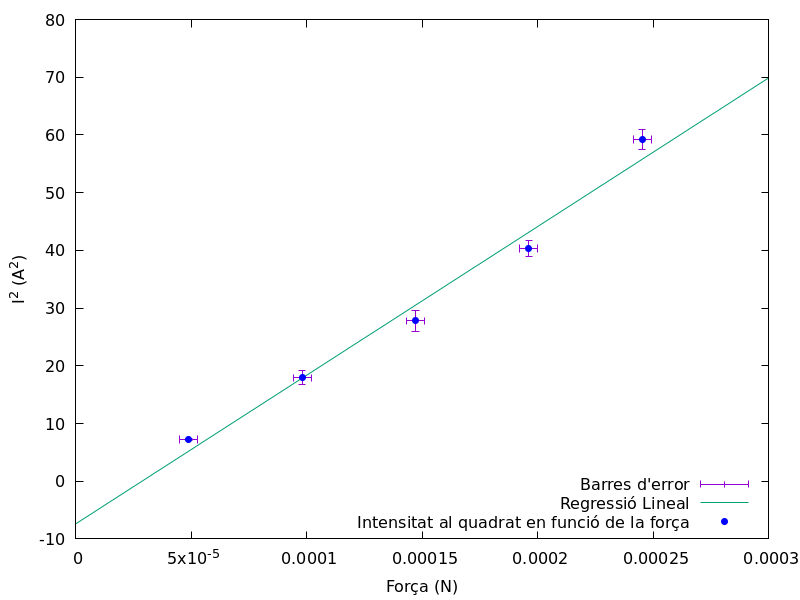
\includegraphics[width=0.5\textwidth]{PR2_regr_I2vsF.png}
    \caption{El quadrat de la intensitat en funció de la Força.}
    \label{fig: PR2_regr_I2vsF}
\end{figure}

La regressió té un coeficient de correlació de $R^2 = 0,9806$. Així doncs, la força que un fil que transporta una intensitat I rep generat pel camp magnètic produit per un altre fil situat paral·lelament i en les mateixes condicions de corrent és proporcional al quadrat de la intensitat: $F \sim I^2$.

El pendent de la recta de regressió ens permet trobar un valor aproximat de $\mu_0$. A partir de l’Eq. \eqref{eq: PR2_Fm_entre_fils} es dedueix que el pendent m serà $m = \frac{2\pi d}{\mu_0 L}$.
Aïllant $\mu_0$ s’obté $\mu_0 = (0,413 \pm 0,091) · 10^{-6}\, T · m/A$, que difereix bastant (tot i tenir el mateix ordre de magnitud) del valor tabulat que hem pres, de $4\pi \cdot 10^{-7}\, T \cdot m/A \,=\, 1,26 \cdot 10^{-6}\, T\cdot m/A$\footnote{Aquest valor tabulat s'ha extret del guió de la pràctica corresponent}. 

Podem veure que el valor teòric no es troba dins de l’interval d’incerteses considerat pel valor experimental i, per tant, els resultats no són compatibles. La incertesa instrumental associada a les mesures, com per exemple, la diferència de massa real respecte la marcada en les etiquetes i el que s'ha utilitzat per fer les regressions fa augmentar la discrepància entre els resultats. 

\subsubsection{Dependència de la força mangètica amb la distància de separació entre fils}\label{sec: PR2_Fm_sep}

En aquest segon apartat analitzarem com depèn la força magnètica amb la distància de separació entre fils per on circula corrent. 

Ho farem aconseguint mantenir en equilibri la força magnètica amb la força de torsió. Així doncs, primer cal obtenir la constant de torsió del fil. Es fixa una intensitat de $(5,00 ± 0,01)$ A i es representen les dades de la força en funció de l’angle. Posteriorment es realitza una recta de regressió que ens permet trobar el valor de la constant $k$.

\begin{figure}[H]
    \centering
    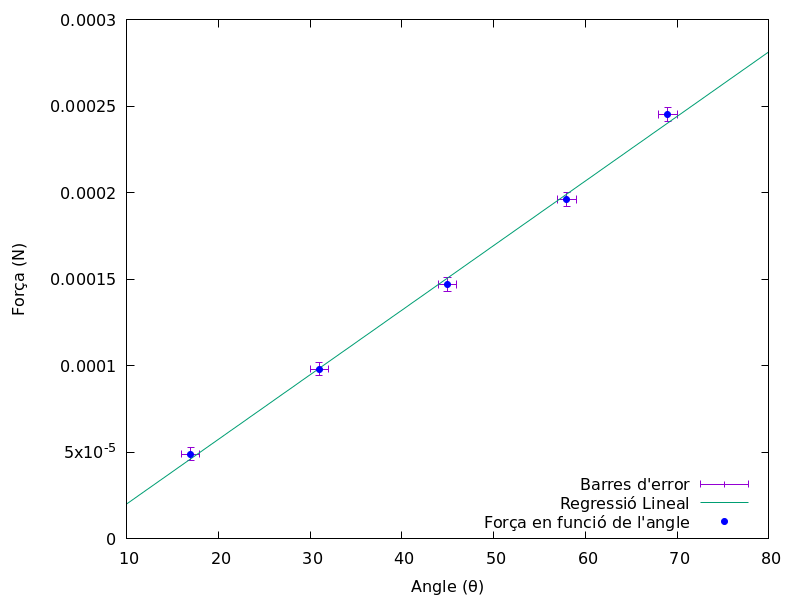
\includegraphics[width=0.5\textwidth]{PR2_regr_Fvstheta.png}
    \caption{Força en funció de l'angle de torsió.}
    \label{fig: PR2_regr_Fvstheta}
\end{figure}

La força que s’obté a partir de la regressió és:

\begin{equation}\label{F_ktheta}
    F(\theta) = (3,73 \pm 0,10) \cdot 10^{-6}\, \theta
\end{equation}

Cal remarcar que la regressió lineal posseeix una ordenada a l’origen llunyana al zero ($(-1,75 \pm 0,50)·10^{-5}$). Tot i que aquesta ordenada d’origen no és menyspreable enfront dels valors de la força, podem no tenir-la en compte ja que aquesta ordenada a l'origen pot haver aparegut a causa d’una imprecisa cal·libració de la balança. A més a més, el fet que la constant de torsió sigui positiva és un bon indicatiu, perquè la força ha d’augmentar linealment amb l’angle de torsió.

A continuació, mantenint fixa la intensitat anterior, es va variant la distància entre ambdós fils de corrent per calcular el valor de la permeabilitat magnètica $\mu_0$. 

Es representen els resultats obtinguts en la Fig. \ref{fig: PR2_regr_thetavsr} on es grafica la força respecte $1/r$:

\begin{figure}[H]
    \centering
    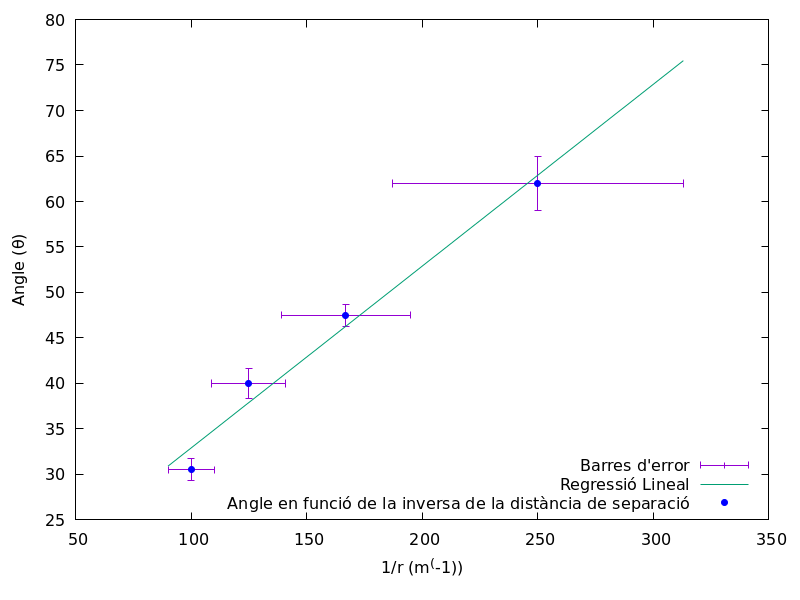
\includegraphics[width=0.5\textwidth]{PR2_regr_thetavsr.png}
    \caption{Força en funció de l’invers de la distància de separació entre fils de corrent.}
    \label{fig: PR2_regr_thetavsr}
\end{figure}

La regressió té un coeficient de correlació de $R^2 = 0,9762$.
Aplicant la relació \eqref{F_ktheta} a l'equació que acabem de trobar i operant, s’obté que el valor de $\mu_o$ ve donat per l’equació $\mu_0 = \frac{2\pi m}{LI^2}$ on $m$ correspon al pendent de la regressió lineal. 

Aplicant el valor experimental s’obté que: $\mu_0 = (0,525 \pm 0,058) \cdot 10^{-6}\, N/A^2$. Tot i que el resultat tampoc és compatible amb l’esperat, sí és molt similar al resultat experimental de l’apartat anterior (tenint en compte els seus intervals d'incertesa, sí són compatibles) . 

De nou, cal considerar que la discrepància és deguda a la complexitat en la mesura de les dades. Un error tan gran pot ser degut a factors que han influït en la mesura i que no s’han pogut tenir en compte en el càlcul de la incertesa, com ara petites vibracions de la taula o una calibració imprecisa de la balança. De fet, tenir aquesta mateixa discrepància en els dos càlculs de la permeabilitat magnètica al buit pot ser un indicatiu que la balança no estava ben calibrada, per això les dependències entre magnituds són correctes, però els valors calculats no. Tanmateix, el resultat és força proper al valor real.

Per millorar l'experiment i que els resultats numèrics fóssin més propers al teòric caldria considerar que la posició d'equilibri es devia trobar desplaçada del zero. També es podria recalibrar la balança de nou per no seguir arrossegant aquest error. Això és el que vam realitzar abans de començar la mesura del camp magnètic terrestre en la secció que ve a continuació.

\subsubsection{Camp magnètic terrestre}\label{sec: PR2_Bterra}

En aquesta última part de la pràctica es pretén mesurar la component horitzontal del camp magnètic terrestre. 

Fixant la intensitat a $(8,00 \pm 0,01)\,A$, trobem el valor de l'angle que permet tornar a deixar en l'equilibri la balança, és a dir, igualem la força que rep el fil degut al camp magnètic amb la de torsió. La torsió obtinguda experimentalment és de $(19,5 \pm 2,3)º$. 

Aprofitant el resultat de la constant de torsió trobada en la Sec. \ref{sec: PR2_Fm_sep}, podem trobar que la força magnètica que s’ha obtingut és de $F = (7,28 \pm 0,90) \cdot 10^{-5}\,N$. 

De l’Eq \eqref{eq: PR2_Fmagn_en_funcio_B}, podem aïllar $B$ i obtenir que la component horitzontal del camp magnètic de la Terra al laboratori de la Universitat Autònoma, és $B = (3,08 \pm 0,59)·10^{-5}\,T$. El valor real que hem agafat és de $B = 2,53·10^{-5}\,T$ \footnote{Valor obtingut d'un document de la R.S.E.F. on s'havia mesurat la component horitzontal del camp magnètic a Salamanca}. Per tant, com el valor experimental es troba dins l’interval d’incerteses, és compatible amb el resultat esperat.

Només hem pogut estudiar la component horitzontal del camp magnètic terrestre perquè la component vertical d’aquest és perpendicular al conductor i, per tant, la balança que tenim no permet fer la seva mesura.

També podem observar que el fet d'haver desplaçat la balança, ens ha obligat a recalibrar aquesta de nou. Això pot haver influit en què els resultats de càlcul del camp magnètic sí continguin el valor teòric en el seu interval d'incerteses.

\subsection{Conclusions}\label{sec: PR2_concl}

En vista dels resultats es comprova que la dependència en $I^2$ i en $1/r$ de la força magnètica, efectivament és lineal, tal com predien les equacions trobades per un sistema de fils paral·lels pels quals circula una mateixa intensitat. 

També s’ha obtingut experimentalment el valor de $\mu_0$ de dues maneres diferents, obtenint en ambdós casos valors que discrepen amb el valor teòric acceptat però similars entre ells.

Concloem doncs, que el mètode experimental és prou bo tot i els errors que té associats. No obstant, veiem que el calibratge inicial de balança és molt determinant en els resultats numèrics, en el nostre cas, s'hauria de tenir en compte que el punt d'equilibri de la balança es trobava fora del zero o es podria haver recalibrat la balança de nou abans de començar a fer les mesures de cada part de l'experiment.

La component horitzontal del camp magnètic terrestre a la Universitat Autònoma és de $B_{T_{norm}}= (3,08 \pm 0,59)\cdot10^{-5} \, T$ que conté dins del seu rang d’incertesa el valor teòric mesurat a Salamanca (el qual utilitzem de referència).

\newpage

\section{\huge \textbf{Pràctica 6}}  % Títol petit en negreta

\vspace{.5em}  % Espai vertical

{\Huge \textbf{Feixos de raigs catòdics}}  % Títol gran

\begin{abstract}
     En aquesta pràctica s'estudia el comportament d'un feix de raigs catòdics sota un camp elèctric i un camp magnètic amb l'objectiu de determinar les propietats de les partícules que els conformen. Concretament, analitzant les desviacions del feix dels raigs sota aquests camps s'obté la relació entre la càrrega i la massa de les partícules que ens permet determinar que són electrons.
\end{abstract}

\subsection{Introducció Teòrica}
En aquesta pràctica estudiarem com es desvia el feix de raigs catòdics sota el camp elèctric generat per un condensador i el camp magnètic generat per unes bobines de Helmholtz. A través de les equacions d'aquests, podrem determinar propietats de les partícules que conformen els raigs. Concretament, els objectius que ens plantegem són:

\begin{list}{$\ast$}{\leftmargin=1em}
    \item Caracteritzar el camp elèctric generat pel condensador no ideal que usem a l'experiment a través d'un factor experimental.
    \item Determinar i explicar el comportament dels raigs catòdics sota el camp elèctric i el camp magnètic. Estudiar-ho per diferents intensitats i potencials aplicats als generadors de camp.
    \item Determinar, amb dos mètodes diferents, de què estan fets els raigs catòdics trobant la relació entre la càrrega i la massa de les seves partícules.
\end{list}


%DESV E
Primerament, estudiarem la desviació del feix deguda a un camp elèctric perpendicular a la velocitat; aplicant una diferència de potencial $V_p$ entre dues plaques plano-paral·leles. Degut a què la distància entre plaques $d$ (= 54 mm) és de l'ordre del tamany d'aquestes, no podem considerar el sistema com un condensador de plaques plano-paral·leles ideal amb un camp uniforme $E=V/d$. En comptes, seguirem considerant-lo uniforme però modificarem l'expressió mitjançant una constant $k$ que tindrà en compte els efectes de vorada i que trobarem experimentalment.
\begin{equation}
    E = \frac{kV_p}{d}
    \label{eq: Camp E}
\end{equation}

Si les partícules de les quals està format els raigs catòdics (de massa $m$) tenen càrrega elèctrica $q$, aquestes es desviaran cap a un dels dos elèctrodes; al càtode si són negatives i a l'ànode si són positives. I la trajectòria que seguiran serà una paràbola parametritzada per l'Eq. (\ref{eq: trajectoria}), ja que el camp és uniforme i en direcció $y$.
\begin{align}    \label{eq: trajectoria}
    &x = v_0 t      &y = -\frac{qEt^2}{2m}
\end{align}

On $v_0$ és la velocitat en direcció $x$ que tenen inicialment les partícules al sortir del filament.
Donat que un cop emeses les partícules, aquestes es veuen accelerades degut al voltatge aplicat $V_a$; per conservació de l'energia, la velocitat ha de ser:
\begin{equation}
    \frac{1}{2}mv_0^2=qV_a
    \label{eq: Energia}
\end{equation}

Tot i això, no es pot veure el moviment d'una partícula individual en funció del temps, sinó que es veu una corba formada per moltes partícules en diferents moments de la trajectòria. L'expressió d'aquesta corba com una funció de $x$ ($y$ = $f(x)$)  s'obtè combinant les Eqs. (\ref{eq: Camp E}), (\ref{eq: trajectoria}) i (\ref{eq: Energia}):
\begin{equation}
    y = \frac{kV_px^2}{4dV_a}
    \label{eq: parabola}
\end{equation}

Per últim, queda determinar experimentalment la constant $k$ a partir del pendent $m$ de la recta de regressió lineal de $y$ en funció de $x^2$ i de l'Eq. (\ref{eq: parabola}):
 \begin{equation}
      k =\frac{4mdV_a}{V_p}
      \label{eq: k}
 \end{equation}

%DESV M
\vspace{1cm}
Per altra banda, estudiarem la desviació del feix deguda a un camp magnètic perpendicular per calcular el radi de corvatura i posteriorment la relació $\frac{q}{m}$ de les partícules dels raigs catòdics. Per això necessitem caracteritzar la trajectòria de les partícules carregades sota un camp magnètic uniforme. En l'experiment, el camp d'inducció magnètica està generat per unes bobines de Hemholtz que aproximadament produeixen el camp uniforme 
\begin{equation}
    \vec{B}=\frac{32\pi nI}{5\sqrt{5}r}\cross10^{-7} \quad \hat{z}\quad Wb/m^2.
    \label{eq: B}
\end{equation}
A més a més, la llei de Lorentz dicta que una partícula carregada negativament sota un camp d'inducció magnètica, $\vec{B}$, pateix una força
\begin{equation}
    \vec{F}=q\vec{v}\cross\vec{B}.
    \label{eq: Lorentz} 
\end{equation} 
En el nostre cas, $\vec{v}$ és perpendicular a $\vec{B }$ i, per tant, les partícules dels raigs catòdics seguiran una trajectòria circular d'equació
%Aquesta força, al ser sempre perpendicular a la velocitat i tenint en compte que en el nostre sistema la velocitat de les partícules carregades, $\vec{v}$, és perpendicular a $\vec{B }$ induirà un moviment circular a les partícules de radi R. La trajectòria de les partícules carregades del nostre sistema complirà
\begin{equation}
    R=\frac{x^2+y^2}{2y}.
    \label{eq: radi}
\end{equation}
On $R$ és el radi del cercle i hem agafag el centre de coordenades a l'inici del tub de raigs catòdics i l'eix $X$ del sistema paral·lel a la direcció de sortida dels raigs.

Ara, per calcular la relació entre la intensitat de corrent de les bobines de Helmoholtz i el radi de corvatura de les partícules cal igualar la força centrípeta a la força de Lorentz, i obtenim 
\begin{equation}
    Bqv=\frac{mv^2}{R}
    \label{eq: fc=fl}
\end{equation}
que combinada amb l'Eq. (\ref{eq: B}) ens dona la relació entre el radi i la intensitat de corrent
\begin{equation}
    R=K\frac{1}{I} \quad on \quad K=\frac{mv5\sqrt{5}r}{32\pi n}\cross 10^7.
    \label{eq: IvsR}
\end{equation}
Tenint en compte l'Eq. (\ref{eq: fc=fl}) i la llei de la conservació de l'energia mecànica, $qV_a = \frac{1}{2}mv^2$, s'obté 
\begin{equation}
    \frac{q}{m}=\frac{2V_a }{B^2R^2}
    \label{eq: q/m}
\end{equation}
que ens permetrà calcular la relació $\frac{q}{m}$ de les partícules.


\vspace{1cm}

Una altre manera de calcular la relació càrrega/massa de les partícules dels raigs catòdics és igualant forces elèctriques i magnètiques. Fent-ho, arribem a la següent equació:

\begin{equation}\label{eq: Fm=Fe}
    qE = qvB
\end{equation}

Amb la que es troba que la velocitat vindrà donada pel quocient:

\begin{equation}
    v = \frac{E}{B}
\end{equation}

Podem obtenir el radi de la trajectòria circular deguda només a la desviació magnètica com hem explicat prèviament.

De les Eqs \eqref{eq: Fm=Fe}, \eqref{eq: fc=fl} es pot deduir l'equació que emprem en la secció \ref{sec: desv_em} per a calcular la relació càrrega/massa a partir de les nostres dades experimentals:

\begin{equation}
    \frac{q}{m}=\frac{E}{RB^2}=\frac{kV_p}{dK^2I^2R}
\end{equation}

\newpage
\subsection{Mètode Experimental}

El procediment experimental seguit ha constat de diversos passos que estan explicades detalladament al guió de la pràctica.

Primerament, s'ha aplicat una diferència de potencial al tub de raigs catòdics i s'ha fet visible el feix lluminós dels raigs. És de gran importància assegurar-se que la connexió per aplicar la diferència de potencial sigui correcta ja que una equivocació entre l'ànode i el càtode provocaria que el raig catòdic es disparés en sentit contrari al que volem, danyant el sistema que permet generar aquests feixos.

La desviació d'aquest feix s'ha estudiat al aplicar diferents valors de camp elèctric (generat per un condensador planoparal·lel) o magnètic (generat per unes bobines de Hemholt) ambdós considerats uniformes i perpendiculars. Per poder determinar punts de la trajectòria del feix de raigs catòdics, hem fotografiat el raig usant un dispositiu mòbil i cobrint-nos amb un material opac per tal de tenir més contrast i poder difernciar-lo bé.

Posteriorment s'ha processat cada imatge a ordinador fent ús del programa $Aseprite$ que permet obtenir punts del feix mitjançant la conversió de pixels a distància en cada fotografia. És a dir, comptant els píxels i convertint-los a centímetres. D'aquesta manera hem pogut obtenir dades numèriques amb les quals es poden trobar paràmetres que poden ser comparats amb valors teòrics tabulats i comprovar així l'eficiència del nostre mètode experimental.

Per estudiar la desviació electroestàtica, s'ha aplicat unes diferències de potencials ($2\,kV, 3\,kV, 4\,kV$ i $5\,kV$) entre les plaques planoparal·leles. Per a la desviació magnetoestàtica, s'analitza el comportament del feix per a un rang d'intensitats ($0.1\,A, 0.2\,A, 0.3\,A, 0.4\,A, 0.5\,A, 0.6\,A, 0.7\,A, 0.8\,A$) i es troba la relació entre el radi de curvatura del feix i la intensitat de corrent de les bobines de Helmholtz. Per últim, en l'estudi de la desviació electromagnètica es busca quina diferència de potencial és necessita per a que el camp elèctric i el d'inducció magnètica mantinguin una trajectòria rectilínia del feix. Tot i que la trajectòria no és perfectament rectilínia per cap valor de potencial, hem agafat com a correcta aquella que presenta menys defelxió i coincideix més amb l'eix d'abscisses en els extrems.

%Aquest doncs, ha estat el procediment seguit: triar a consciència diversos punts del feix i donar-ne la posició (x,y) més exacta possible, sempre sent possibles errors degut al processat de la fotografia o al desplaçament de píxels. Més precisament, s'ha aplicat una grid (cuadrícula) sobre els espais compresos entre cada marca de la regla, coincidint amb cada variació de 1 cm, per cada eix. Així, per cada una de les imatges s'ha establert una conversió píxel/cm. S'inclou un exemple gràfic (\ref{fig: ex_grid}) a continuació:

%\begin{figure}[H]
  %  \centering
   % 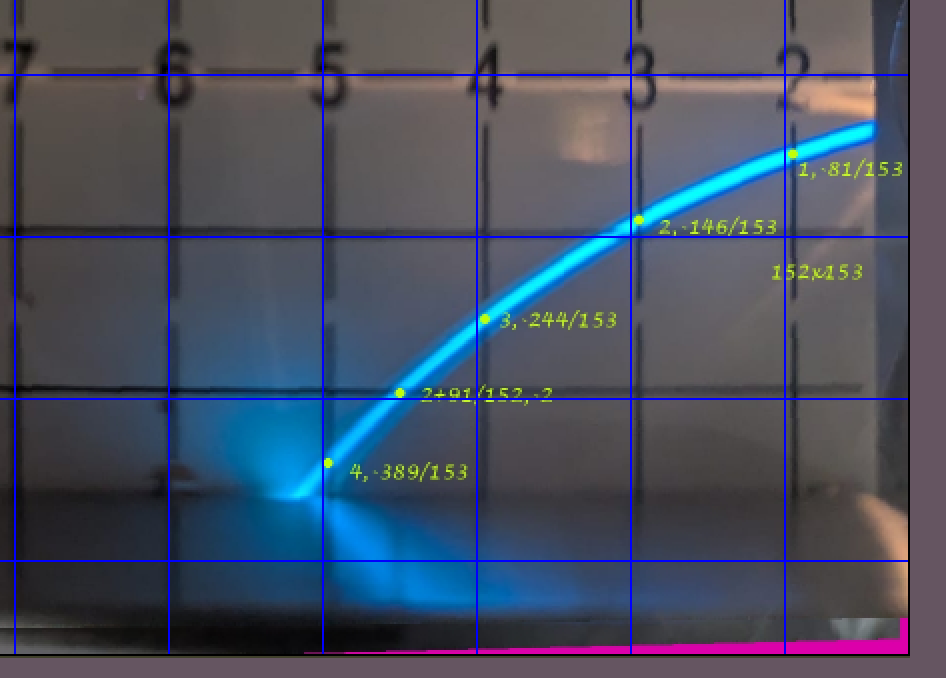
\includegraphics[scale=0.3]{Ex_grid.png}
    %\caption{Imatge modificada després de l'aplicació de la grid %corresponent amb la seva relació px/cm: 152/1 i 153/1.}
    %\label{fig: ex_grid}
%\end{figure}

%Llavors, per cada un dels punts s'ha determinat la posició dins la grid comptant els píxels de separació amb la frontera del quadrat corresponent, i finalment, s'han convertit a centímetres. Amb aquests resultats, s'ha estudiat la desviació de la trajectòria; fet crucial pel desenvolupament de la prova, doncs les partícules del feix es poden identificar segons aquest comportament.

\newpage
\subsection{Resultats i discussió}

\subsubsection{Desviació electroestàtica}\label{sec: desv_electr}

En subministrar una diferència de potencial a les plaques s'observa com el raig es desvia cap al càtode\footnote{Les imatges de la desviació electroestàtica (Fig.(\ref{fig: Desv E})) es troben a l'annex (\ref{sec: imatges}) }. Per tant, les partícules de les què està compost els raigs catòdics tenen una càrrega negativa.

 Per comprovar que les trajectòries es tracten de paràboles hem fet una regressió de les $y$ en funció de les $x^2$, com es mostra a la figura (\ref{fig: Regressió Desv E}). Aquestes tenen els següents coeficients de correlació \footnote{Les regressions lineals en detall es troben a l'annex \ref{sec: Ap_Regr}}:
 r$^2$ = 0.9777, 0.9973, 0.9940, 0.9832. Confirmant que les partícules segueixen una trajectòria parabòlica i, per tant, el camp elèctric generat pel condensador es pot considerar uniforme; tal com haviem proposat. 
\begin{figure}[H]
    \centering
    \begin{minipage}{0.75\textwidth}
    \centering
        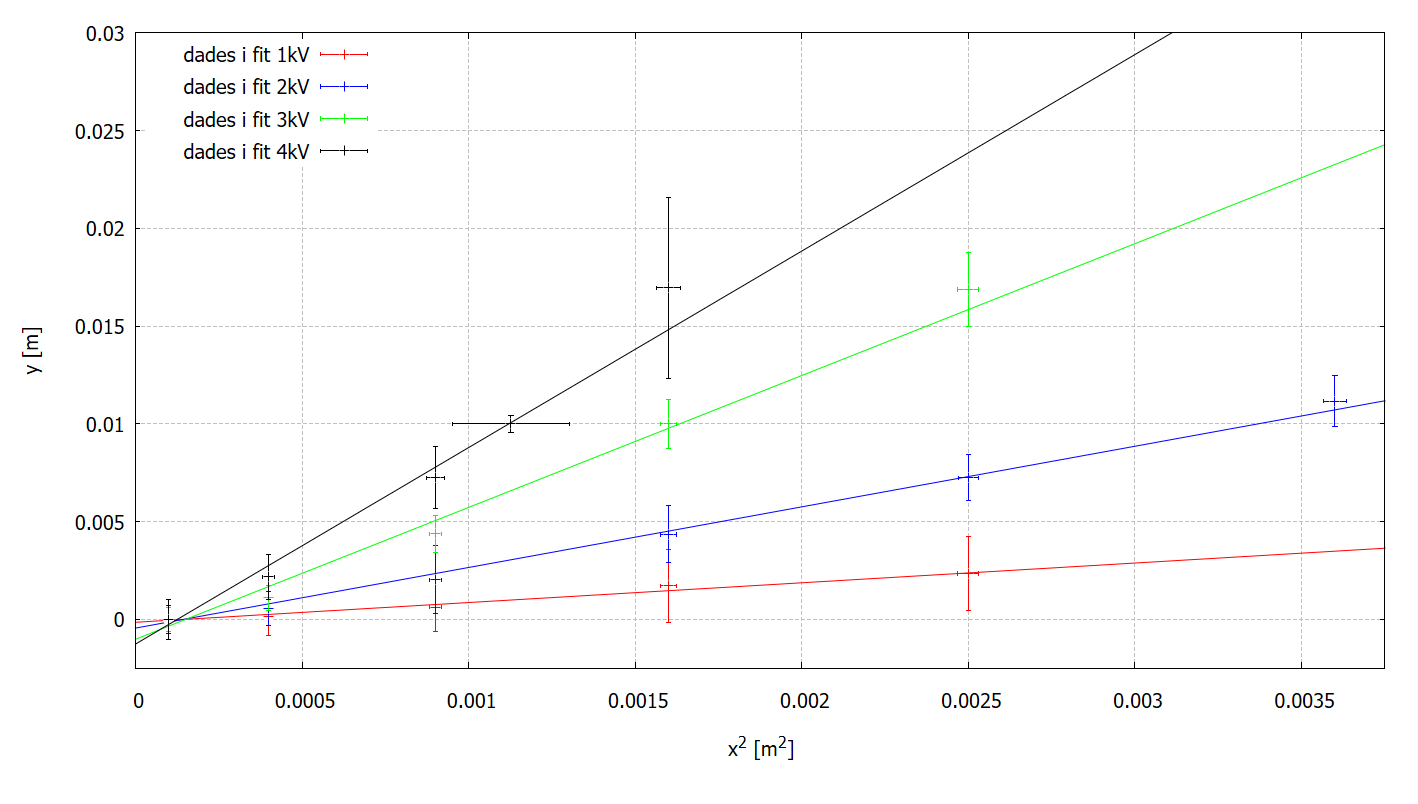
\includegraphics[width=1\linewidth]{Plot yvsx.PNG}
        \caption{Regressió de $y$ en funció de $x^2$  de la desviació deguda al camp elèctric}
        \label{fig: Regressió Desv E}
    \end{minipage}
\end{figure}

A la taula \ref{tab:kvsVp} podem observar els diferents valors que pren $k$ \footnote{El càlcul de les incerteses es mostra a l'anex \ref{sec: incerteses}} en funció del potencial entre plaques $V_p$, obtinguts a partir del pendent d'aquestes regressions lineals juntament amb l'Eq. (\ref{eq: k}). Observem que la $k$ no és constant i que augmenta amb la diferència de potencial. Fent una regressió lineal entre $V_p$ i $k$ obtenim que hi ha una relació lineal entre els dos amb un coeficient de correlació r$^2$ = 0.9737 i una equació de la recta: $k = 0.453 \cdot 10^{-3}\, V^{-1}  \cdot V_p + 0.45$.

Aquests resultats ens indiquen que, per als voltatges de 2 kV, 3 kV i 4 kV, el valor del camp elèctric (en la regió dins del condensador) és major que el camp elèctric que generaria un condensador de plaques plano-paral·leles ideal. Aquest resultat és contradictori perquè el potencial entre plàques és $V_p \equiv \Delta V = \int\vec{E}\cdot\vec{dl}$, on hem suposat que el camp $\vec{E}$ té mòdul constant. Escollint el camí amb direcció tangencial al camp elèctric: $V_p = E \cdot l\ge E\cdot d = kV_p > V_p$. No només això, les dades també indiquen que el camp elèctric depèn quadràticament del potencial de les plàques. Sabem que aquest resultat és incompatible amb la teoria; ja que, donades unes condicions de contorn del potencial $V(\vec{r)}$ i la solució de l'equació de Laplace $\phi(\vec{r})$ i $\vec{E}(\vec{r})$ , la solució per a unes condicions proporcionals $V'(\vec{r)}=\lambda V(\vec{r)}$ és també proporcional $\phi'(\vec{r}) = \lambda \phi(\vec{r})$ i $\vec{E}'(\vec{r}) = \lambda \vec{E}(\vec{r})$.

\begin{figure}[H]
    \centering
    \begin{minipage}{0.45\textwidth} 
        \centering
        \begin{tabular}{|c|c|}
            \hline
            $V_p$ (V)	&	$k$	\\\hline
            (1000 ± 200)	&	(0.87 ± 0.64)   \\\hline
            (2000 ± 200)	&	(1.35 ± 0.22)	\\\hline
            (3000 ± 200)	&	(1.94 ± 0.25)	\\\hline
            (4000 ± 200)	&	(2.17 ± 0.26)	\\\hline           
        \end{tabular}
        \captionof{table}{Resultats experimentals de les constants $k$ del condensador per cada valor del potencial $V_p$.}
        \label{tab:kvsVp}
    \end{minipage}
\end{figure}

Aleshores, podem deduir que la constant $k$ no és una constant que modifiqui directament el camp elèctric $E$, sinó que la constant $k$ ens permet representar el sistema com un condensador de plaques plano-paral·leles ideal amb una diferència de potencial $k V_p$. 

\subsubsection{Desviació magnetoestàtica}\label{sec: desv_magn}
Després de comprovar a la Secció \ref{sec: desv_electr} que les partícules dels ràigs catòdics tenen càrrega negativa, n'estudiarem la interacció amb el camp magnètic, substancialment uniforme, generat per unes bobines de Helmholtz. 
Al aplicar el camp, com era d'esperar, hem observat que els ràigs es corbaven i ens hem disposat a estudiar les dependències d'aquesta corba i el seu radi amb la intensitat del corrent de les bobines i amb el potencial dels raigs catòdics.

Per calcular el radi de la trajectòria de les partícules dels raigs catòdics en funció de la intensitat de corrent de les bobines hem usat l'Eq. (\ref{eq: radi}) que defineix el radi com el pendent de la recta de regressió entre $x^2+y^2$ i $2y$. A la Fig. (\ref{fig: regressio_1}) hem representat una selecció d'aquestes regressions i ja podem veure com, a mesura que augmenta la intensitat, el pendent de la recta, és a dir, el radi de les partícules, disminueix. 
\begin{figure}[H]
    \centering
    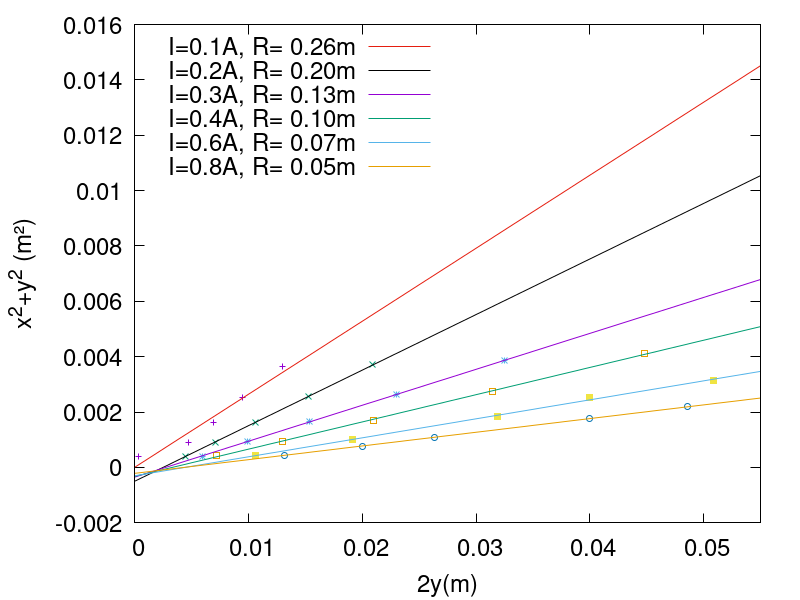
\includegraphics[scale=0.3]{regressio_1.png}
    \caption{Regressió per diverses intensitats de les bobines de Hemholtz de $x^2+y^2$ en front $2y$ on $y$ i $x$ són punts de la trajectòria dels raigs catòdics. La pendent de les rectes és el radi de corvatura de la trajectòria.}
    \label{fig: regressio_1}
\end{figure}
Aplicant diverses intensitats a les bobines de Helmholtz hem obtingut els radis de corvatura de la Taula \ref{tab:RvsI} que es pot trobar a l'annex conjuntament amb el càlcul d'incerteses. Amb aquestes dades (excloent l'última dada ja que té massa incertesa a causa de l'amplada del feix dels raigs) hem construit la gràfica de la Fig. (\ref{fig: RvsI}) on es mostra que la variació del radi corvatura és lineal amb la variació de la inversa de la intensitat. 
Al fer la regressió lineal del radi en funció de l'inversa de l'intensitat hem obtingut la recta
\begin{equation}
    y=x(0.03976\pm0.0006)+(0.0002\pm0.0016)
\end{equation}  
amb un coeficient de determinació de $r^2\approx0,9989$. Per tant, la relació és certament lineal tot verificant la predicció de l'Eq.(\ref{eq: fc=fl}) ja que a més a més, l'ordenada a l'origen inclou el zero. El radi de corvatura és inversament proporcional a la intensitat a causa de què al augmentar la intensitat de les bobines de Helmholtz el camp d'inducció magnètica augmenta provocant que les partícules rebin més força centrípeta què alhora provoca que el radi de la trajectòria disminueixi.
\begin{figure}[h]
    \centering
    \begin{minipage}{0.45\textwidth}
        \centering
        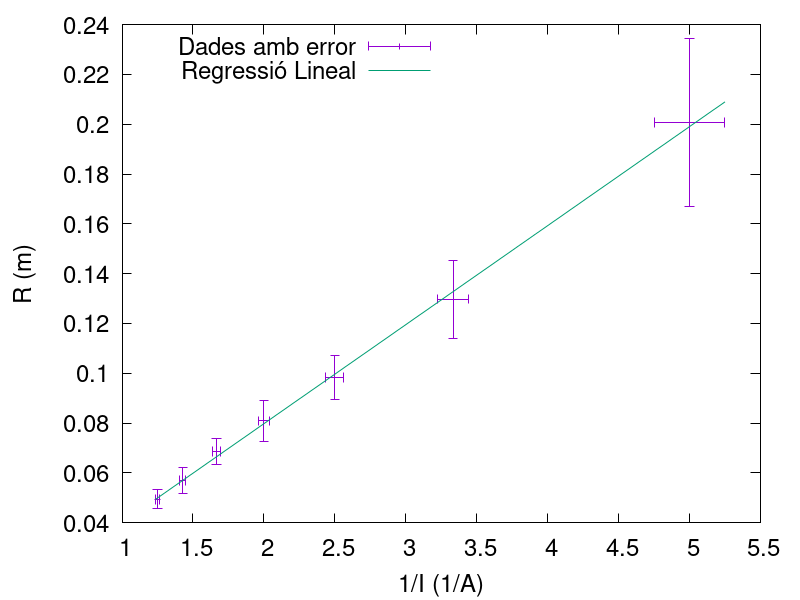
\includegraphics[width=\textwidth]{RvsI.png}
        \caption{Regressió de R en funció de $1/I$ excloent l'últim punt que perd la tendència.}
        \label{fig: RvsI}
    \end{minipage}
    \hfill
    \begin{minipage}{0.45\textwidth} 
        \centering
        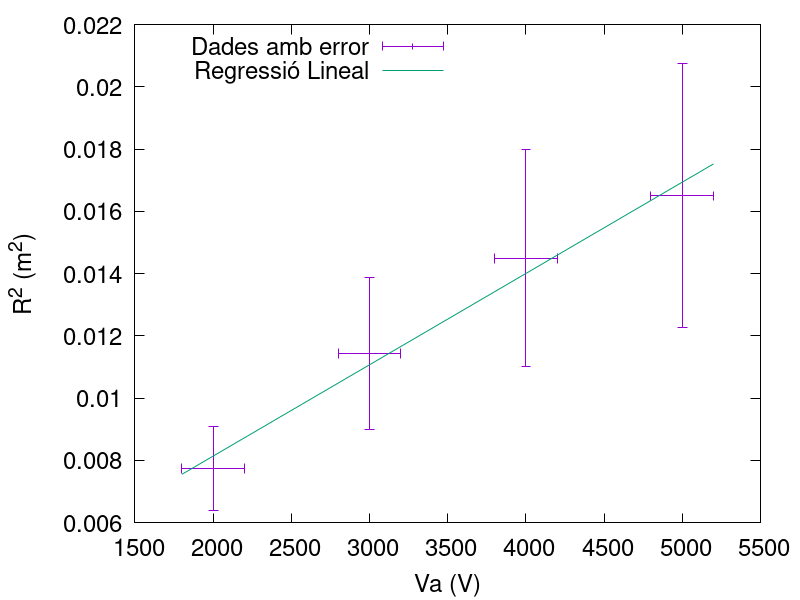
\includegraphics[width=\textwidth]{RvsVa.png}
        \caption{Regressió dels punts experimentals de $R^2$ en funció de $V_a$. Veiem que la relació és clarament lineal.}
        \label{fig: RvsVa}
    \end{minipage}
\end{figure}
Per calcular el radi de la trajectòria de les partícules dels raigs catòdics en funció del potencial d'acceleració d'aquestes usem l'Eq. (\ref{eq: radi}) que defineix el radi com el pendent de la recta de regressió entre $x^2+y^2$ i $2y$. Alicant diferents potencials a les bobines de Helmholtz s'obtenen els radis de corvatura de la Taula \ref{tab:RvsVa} que es troba a l'Annex. Amb aquestes dades hem construit la gràfica de la Fig. (\ref{fig: RvsVa}) on es mostra que la variació de $R$ és quadràtica amb la variació de $V_a$. Al fer la regressió lineal de $R^2$ respecte $V_a$ hem obtingut la recta
\begin{equation}
    y=x(2.93\times10^{-6}\pm0.27\times10^{-6})+(2.28\times 10^{-3}\pm9.8\times10^{-4})
\end{equation}  
amb un coeficient de determinació $r^2=0,9965$. Per tant, la relació és certament lineal (quadràtica respecte $R$) i corrobora l'Eq. (\ref{eq: q/m}). Tanmateix, l'ordenada a l'origen no és compatible amb la teoria ja que no inclou l'origen. Aquesta discrepància amb la teoria possiblement es deguda a que hi ha altres factors instrumentals que no hem tingut en compte a la incertesa com la deformació òptica de les fotografies del feix.


Finalment, amb l'Eq. (\ref{eq: q/m}) hem obtingut la relació $\frac{q}{m}$ de les partícules dels raigs catòdics
\[
\boxed{\frac{q}{m}=(-4.16\pm0.88)\cross10^{11}\quad \mathrm{\frac{C}{Kg}.}}
\]
Per fer-ho hem calculat la regressió lineal ajustada entre $2V_a$ i $B^2R^2$. Així, hem obtingut la recta $y=(4.16\pm0.38)x - (1412.64\pm791.71)$ amb un coeficient de determinació de $r^2\approx0,9837$. El pendent d'aquesta recta ens ha donat el valor de $\frac{q}{m}$ i després hem afegit l'insertesa instrumental al resultat. La $r^2$ tant propera a $1$ indica que els nostres resultats concorden amb la teoria ja que com veiem a l'Eq. (\ref{eq: q/m}) la relació ha de ser lineal. 
Per altra banda, el valor tabulat\footnote{Valor obingut de la pàgina del NIST: "The NIST Reference on Constants, Units and Uncertainty".} de la relació $\frac{q}{m}$ dels electrons és de $\frac{q}{m}=(-1.76\times10^{11}\pm5.5\times10^{2}) \frac{C}{Kg}$ que    com podem veure no és compatible amb el nostre resultat però sí que coincideix en ordre de magnitud. Això pot ser per diversoso motius com que, com es veu a la Secció \ref{sec: traj_no_rect} el camp magnètic generat per les bobines de Hemholtz no és del tot uniforme o que el feix dels raigs catòdics té un gruix considerable que fa molt difícil l'obtenció dels punts experimentals.


\subsubsection{Desviació electromagnètica}\label{sec: desv_em}

En aquest tercer apartat ens interessem la relació càrrega/massa de les partícules dels raigs catòdics per a comprovar que aquesta coincideix amb la de l'electró. 

Tenint en compte el que ja hem pogut observar en els apartats anteriors: la desviació parabòlica a l'aplicar un camp elèctric $\vec{E}$ i desviació circular a l'aplicar el camp d'inducció magnètica $\vec{B}$, el que ens interessa en aquest tercer apartat és aplicar els dos camps a la vegada de tal manera que de les dues deflexions estiguin al mateix pla però en amb direccions oposades de manera que aconseguim que la trajectòria dels raig catòdics no es vegi desviada.

Primerament, hem trobat el valor de la diferència de potencial aplicat entre les plaques amb el qual la desviació de la trajectòria rectilina paral·lela a l'eix de les abscisses és mínima. En concret hem hagut d'aplicar una diferència de potencial $Vp = (0,85 \pm 0,20 )\, kV$ per compensar un camp magnètic generat per bobines amb intensitat de $I = (0,10 \pm 0,01 )\, mA$ i un potencial $Va = 3\, kV$ per a l'accelaració de les partícules dels raigs catòdics.

Fixant aquests valors de pontencial i d'intensitat, posteriorment es suprimeix el camp elèctric $\vec{E}$ per poder mesurar el radi de la trajectòria que deguda només de la desviació magnètica d'igual manera que en la secció \ref{sec: desv_magn}.

Amb aquestes dades hem obtingut el radi de la trajectòria pel mètode dels mínims quadrats, on aquest venia donat pel pendent de la recta de regressió lineal.

Essent la recta en qüestió: 
\begin{equation}
    y=(0,244 \pm 0,033)x + (-2,0 \pm 1,3) \times10^{-4}
\end{equation}  
amb un coeficient de determinació $r^2=0.96$ i  donant un resultat de $R = (0.243 \pm 0.039) \, m$.

La constant del condensador $k$, amb valor $(1,06 \pm 0,28)\, V^{-1}$ la qual té en compte els efectes de vorada de les plaques, la hem obteningut com hem fet prèviament a la secció \ref{sec: desv_electr}. 

D'altra banda la constant de les bobines de Hemholtz $K$ ve determinada per la geometria d'aquestes, com s'explica en la secció \ref{sec: desv_magn}.

Per últim, un cop hem trobat la relació càrrega-massa $q/m$\footnote{El càlcul de les incerteses associades a aquest resultat es presenten en l'annex \ref{sec: incerteses}} podem comparar-la amb la relació e/m, on e correspon a la càrrega d'un electró i m a la seva massa.

\[
\boxed{\frac{q}{m}=(-3,8 \pm 1,7)\cdot 10^{11}\, C/Kg.}
\] 

Tot i que coincideix en ordre de magnitud, observem que el nostre resultat q/m queda lluny del resultat que esperàvem. De fet, el valor trobat no arribar a ser compatible amb l'esperat ja que no l'inclou en el seu rang d'incerteses. 

En vistes dels dos resultats de relació càrrega/massa s'hauria de tenir en consideració que el gruix del feix de raigs catòdics s'anava ampliant com més lluny de l'emissor es trobava. Aquest factor sí s'hagués pogut incloure en la incertesa instrumental de les mesures de la trajectòria.

No obstant, la discrepància pot ser deguda a factors que no es poden incorporar en les incerteses de les mesures. Per exemple, cal notar que la trajectòria mesurada no és perfectament rectilínia tot i haver-se considerat així per poder fer el càlcul de la relació càrrega/massa. De fet, la trajectòria no és o com aquella que podem observar quan no hi ha aplicat cap camp, ni camp elèctric ni camp magnètic, la qual s'apropa molt més a una linia horitzontal constant al llarg de tot el feix observable. 

Això és degut a la no uniformitat que s'ha suposat en el tractament matemàtic tant del camp elèctric com del camp magnètic. Per una banda el condensador no és ideal, ja que les plaques són petites, lluny de poder-se considerar infinites però és cert que aquests efectes de vorada ja els tenim en compte al calcular la seva $k$ mitjançant la regressió lineal. D'altra banda, el solenoide emprat no és ideal tampoc, ja que la seva longitud no és molt més gran que el radi. Això implica que el camp en l'interior sigui de magnitud més gran com més aprop de l'eix central de la bobina ens trobem. Aquest és l'efecte que podem observar en les imatges, podem veure com la trjaectòria dels raigs catòdics presenta més desviació deguda al camp magnètic quan passa pel centre del solenoide.

\subsection{Conclusions}
A partir de l'experimentació amb els raigs catòdics, s'han obtingut resultats que confirmen el comportament esperat dels electrons sota la influència de camps elèctrics i magnètics. 
    
En aplicar una diferència de potencial en les plaques del condensador, s'ha observat que el feix de partícules es desvia en la direcció contrària al camp elèctric. Al travessar una regió amb un camp magnètic uniforme, la trajectòria del feix canvia a una corba amb un radi que té dependència inversament proporcional amb el quocient càrrega/massa ($q/m$) i amb la intensitat del camp magnètic. 

Així doncs, s'ha verificat que els feixos tractats, els raigs catòdics, estan compostos per partícules carregades negativament i que efectivament, són electrons. Tanmateix, fixant-nos en les diferències numèriques trobades al comparar els nostres resultats amb els esperats, podem concloure que el disseny experimental és prou bo per a estudiar la relació càrrega/massa de les partícules dels raigs catòdics però no suficientment exacte. Per millorar aquests resultats es podria haver tingut en compte en la incertesa de les mesures que el gruix del feix catòdic s'anava ampliant com més lluny es trobava de l'emissor. 

\newpage

\section{\huge{\textbf{Pràctica 7}}} \label{sec: pràctica 7}

\vspace{.5em}  % Espai vertical

{\Huge \textbf{Camps magnetics despires i bobines}}  % Títol gran

\begin{abstract}
En aquesta pràctica estudiarem el camp d'inducció magnètica generat per espires al seu centre i bobines al seu eix, amb l'objectiu de verificar la llei de Biot-Savart i el principi de superposició. També aprofitarem les mesures del camp en el centre de les espires de diferents radis i nombre de voltes per obtenir la permeabilitat magnètica del buit i comparar-la amb el valor tabulat. Finalment, complementarem els resultats obtinguts amb computacions numèriques del camp d'inducció en una bobina en tot l'espai, que no tenen expressió analítica.
\end{abstract}


\subsection{Introducció}\label{sec: intro}

En aquesta pràctica estudiarem el camp d'inducció magnètica $B$ generat per diferents geometries (espires i bobines). Els objectius que ens plantegem són:

\begin{list}{$\ast$}{\leftmargin=1em}
    \item Comprovar experimentalment la llei de Biot-Savart. Estudiant el camp generat per unes espires al seu centre i les dependències amb el radi i el nombre d'espires. I estudiant el camp generat dins d'una bobina.
    \item Determinar experimentalment la permeabilitat magnètica del buit $\mu_0$.
    \item Comprovar el principi de superposició estudiant diversos sistemes d'espires i bobines amb la mateixa geometria, però amb un major nombre de voltes.
\end{list}

Per tal d'assolir aquests objectius, primer cal saber quina és la llei de Biot-Savart i quins camps resulten d'ella per a espires i bobines.

La llei de Biot-Savart és:
\begin{equation} \label{eq: Biot-Savart}
    \vec{B}(\vec{r}) = \frac{\mu_0}{4\pi}\int_V\frac{\vec{J}(\vec{r'}) \cross (\vec{r}-\vec{r'})}{\abs{\vec{r}-\vec{r'}}^3}d^3r'
\end{equation}

Aplicant-la per obtenir el camp al centre d'una espira i en l'eix d'una bobina, tenim respectivament:
\begin{equation} \label{eq: B_espira}
    \vec{B} = \frac{\mu_0IN}{2R}\hat{z}
\end{equation}
\begin{equation} \label{eq: B_bobina}
    \vec{B} = \frac{\mu_0IN}{2L}\left(\frac{x-L/2}{\sqrt{R^2+(x-L/2)^2}}-\frac{x+L/2}{\sqrt{R^2+(x+L/2)^2}}  \right) \hat{z}
\end{equation}

On $I$ és la intensitat que circula, $N$ és el nombre de voltes que té l'espira o bobina, $R$ és el radi de l'espira o bobina i $L$ és la longitud de la bobina.

\subsection{Mètode experimental}\label{sec: mètode}

\underline{Muntatge experimental:}
Per dur a terme els experiments, hem muntat el circuit que es mostra en la Fig. (\ref{fig: muntatge}). On l'espira o bobina es troba connectada al generador que subministra corrent continu i a un amperímetre en sèrie. És important que l'escala de l'amperímetre estigui en 10A i no deixar la intensitat circulant durant massa temps perquè treballarem a intensitats altes. Alhora, la sonda Hall estarà connectada al teslàmetre i estarà agafada per un suport que permeti moure-la i orientar-la amb facilitat.

En encendre el teslàmetre, cal esperar a que aquest s'estabilitzi el màxim possible al voltant d'un valor; tot i això, el valor sempre oscil·larà al voltant de $\pm$ 2 mT. Seguidament, ajustar el zero. És possible que durant la realització de l'experiment el teslàmetre es descalibri; en aquest cas, caldria tornar a ajustar el zero. Al realitzar mesures amb el teslàmetre, la sonda ha de estar completament alineada amb el camp que es vol mesurar, ja que només mesura la component del camp $\vec{B}$ paral·lela a aquesta.

A l'hora de fer el muntatge per mesurar el camp de les espires, col·loquem l'espira a un suport mòbil com el de la sonda, de manera que la sonda i l'espira es troben a la mateixa alçada, i la connectem al generador. A l'hora de mesurar el camp d'inducció generat per l'espira, la punta de la sonda s'ha de trobar al centre de l'espira. La punta de la sonda es trobarà just al centre si la distància entre la sonda i qualsevol punt de l'espira és igual al radi de l'espira. Alhora, la sonda estarà alineada amb el camp quan es trobi totalment perpendicular al pla de l'espira. 


El muntatge per mesurar el camp de les bobines consisteix en una regla graduada, una sonda col·locada en el suport mòbil i unes bobines, elevades per uns blocs de fusta, i connectades al generador. 
Segons la sonda vagi entrant en la bobina, mesurarem la distància recorreguda per saber en quin punt es troba la punta de la sonda relativa al origen. Escollim l'origen just quan la punta de la sonda es troba a l'extrem de la bobina (la part de plàstic); de manera que la posició de la punta de la sonda serà la distància relativa menys la distància des d'on comencen els cables fins on comença la bobina (plàstic).
Per mesurar el camp d'inducció amb la major precisió possible, ens assegurem que la punta de la sonda es troba en l'eix de la bobina a ull (ja que no és possible fer-ho amb el regle com abans); mirant des d'un extrem de la bobina, evitant al màxim possible l'efecte paral·laxi (parallax en anglès)\footnote{L'efecte parallax és una desviació de la posició aparent d'un objecte respecte un altre, depenent del punt de vista escollit}. Com que la sonda ha de entrar sencera dins de la bobina, aquesta ja estarà alineada.



\begin{figure}[H]
    \centering
    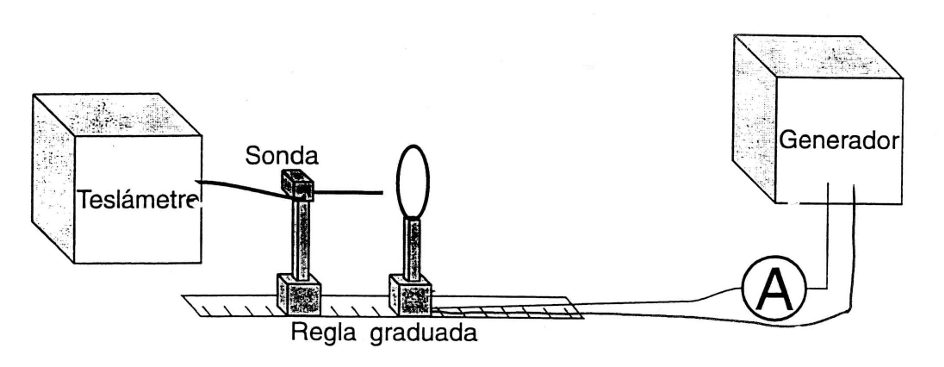
\includegraphics[width=0.75\linewidth]{Muntatge Experimental.png}
    \caption{Muntatge Experimental}
    \label{fig: muntatge}
\end{figure}

Per tal de mesurar únicament el camp generat per les espires o bobines i no cap camp extern. Farem dues mesures del camp però amb la intensitat circulant en sentit oposat. Així, obtenim que el camp generat serà la semidiferència de les dues mesures.
\begin{equation} \label{eq: B_semidif}
    B_{semidif} = \frac{B_+ - B_-}{2}
\end{equation}
D'aquesta manera, qualsevol camp extern que pugui haver-hi (que no variarà en invertir el sentit del corrent), es cancel·larà al fer la resta. És important, pel bon manteniment del generador, cada cop que invertim el corrent; baixar la intensitat a zero,  apagar el generador, canviar els cables i tornar a encendre el generador.

\underline{Obtenció de resultats:} A l'hora d'estudiar el camp generat per una espira (o conjunt d'espires) analitzarem la dependència del camp amb els paràmetres de l'espira mitjançant regressions lineals i el seu coeficient $r^2$. 

La primera dependència que estudiarem serà amb el radi; aquesta, segons la llei de Biot-Savart, ha de ser inversament proporcional. D'aquesta manera, la regressió lineal serà la següent:
\begin{equation}\label{eq: BvsR}
    B=\frac{m}{R} + n
\end{equation}
Per realitzar la regressió, prendrem mesures en tres espires diferents amb radis $R$: 3 cm, 4,25 cm i 6,75cm . I amb la resta de paràmetres fixats: $I=1A$ i $N=1$. 

La segona dependència que estudiarem serà amb el nombre de voltes que té el conjunt d'espires; aquesta, pel principi de superposició, ha de ser proporcional. D'aquesta manera, la regressió lineal serà la següent:
\begin{equation}\label{eq: BvsN}
    B=mN + n
\end{equation}
Per realitzar la regressió, prendrem mesures en tres conjunts d'espires amb diferent nombre d'espires $N$: 1, 2 i 3. I amb la resta de paràmetres fixats: $I=1A$ i $R = 6,75 cm$. 

A partir d'aquestes regressions, a més de confirmar la relació entre el camp i el radi i el nombre d'espires, calcularem la permeabilitat magnètica del buit $\mu_0$ comparant les dues rectes de regressió fetes anteriorment i l'expressió teòrica del camp magnètic:

Comparant les Eqs. (\ref{eq: B_espira}), (\ref{eq: BvsR}).
\begin{align} \label{eq: mu1}
    m = \frac{\mu_0IN}{2}      \nonumber \\
    \mu_0=\frac{2m}{IN}
\end{align}
I comparant les Eqs. (\ref{eq: B_espira}), (\ref{eq: BvsN})
\begin{align} \label{eq: mu2}
    m = \frac{\mu_0I}{2R}        \nonumber \\
    \mu_0=\frac{2Rm}{I}
\end{align}

\subsection{Resultats experimentals}\label{sec: resultats}
\subsubsection{Mesaura del camp de les espires}\label{subsec: espires}

En la Fig. (\ref{fig:BvsR}) es mostren les dades obtingudes experimentalment del camp d'inducció $B$ enfront de l'invers del radi de les espires $1/R$ (en blau) juntament amb el valor teòric que haurien de tenir (en verd) seguint l'Eq. (\ref{eq: B_espira}); es pot observar com les dades experimentals i teòriques són compatibles.
Juntament amb les dades experimentals, la figura presenta una recta de regressió lineal amb un coeficient de correlació \footnote{Les regressions lineals en detall es troben a l'annex \ref{sec: Ap_Regr}} $r^2 = 0,9994$ i amb l'equació: 
\begin{equation} \label{reg: BvsR}
    B = (2,7\pm 1,1) \cdot10^{-6} m\cdot T*\frac{1}{R}+(-3 \pm 28)\cdot10^{-6} \, T
\end{equation}
El coeficient de correlació és suficientment elevat com per confirmar una relació lineal entre el camp $B$ i l'invers del radi $1/R$.
Alhora, l'ordenada a l'origen de l'Eq. (\ref{reg: BvsR}) és $(-3 \pm 28)\cdot10^{-6}$ T essent compatible amb zero; això ha de ser així per què quan $1/R$ és zero, és a dir $R$ tendeix a infinit, és com si no hi hagués cap espira i, per tant, no ha d'haver-hi cap camp. Per tant, confirmem que el camp és inversament proporcional al radi.

Finalment, a partir de la pendent de la recta de regressió de l'Eq. (\ref{reg: BvsR}) i l'Eq. (\ref{eq: mu1}) obtenim la $\mu_0$:

\[
\boxed{\mu_0=(1,35\pm0,55)\cdot10^{-6} \, N/A^2}
\]

El resultat de la permeabilitat magnètica del buit $\mu_0$ obtingut a partir de la regressió és compatible amb el valor tabulat de $\mu_0 =$  1,25664 $\cdot 10^{-6}$ N/A$^2$ \footnote{El valor tabulat de la permeabilitat magnètica del buit està extreta de: «Convocationde la Conférence générale des poids et mesures (26e réunion)»}.

\begin{figure}[H]
    \centering
    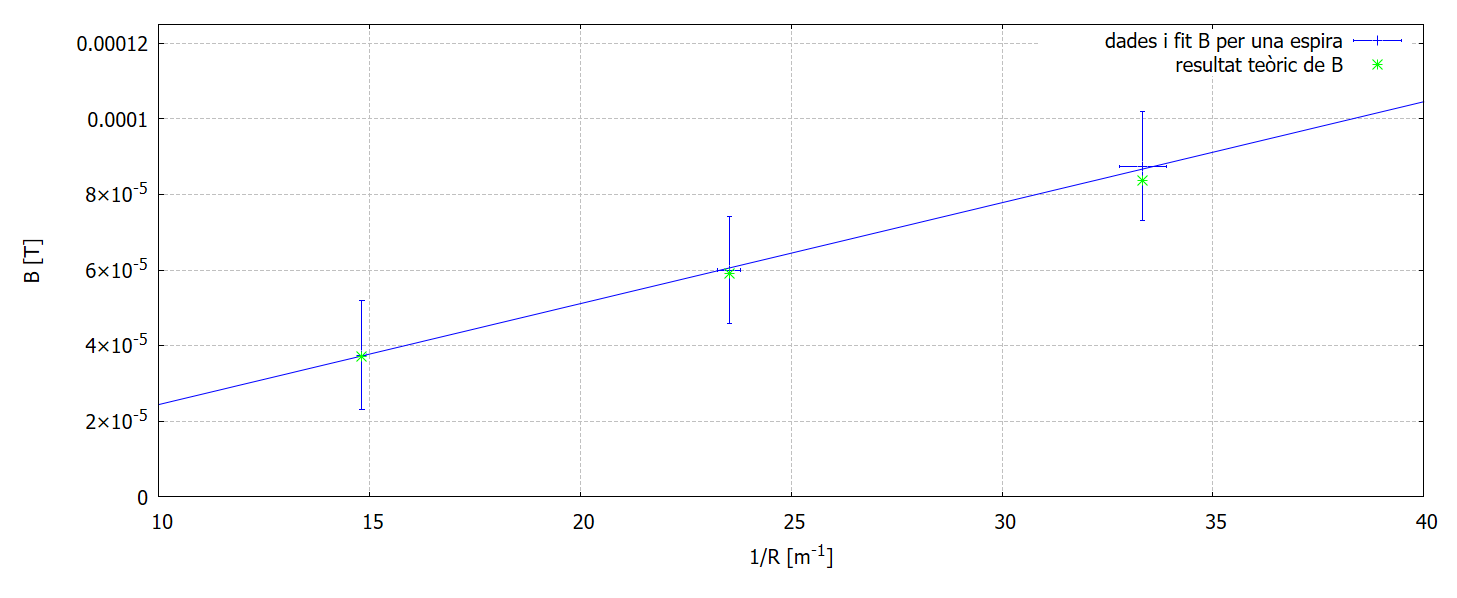
\includegraphics[width=1\linewidth]{BvsR.PNG}
    \caption{Regressió lineal del camp generat $B$ per una espira en el seu centre en funció del invers del seu radi $R$, comparat amb els valors teòrics.}
    \label{fig:BvsR}
\end{figure}

En la Fig. (\ref{fig:BvsN}) es mostren les dades obtingudes experimentalment del camp d'inducció $B$ enfront del nombre d'espires $N$ del conjunt (en blau) juntament amb el valor teòric que haurien de tenir (en verd) seguint la fórmula (\ref{eq: B_espira}); es pot observar com les dades experimentals i teòriques són compatibles.
Juntament amb les dades experimentals, la figura presenta una recta de regressió lineal amb un coeficient de correlació de $r^2=0,9987$ i amb una equació:
\begin{equation} \label{reg: BvsN}
    B = [(4,0 \pm 1,0) \cdot10^{-5} *N +(-3 \pm 22)\cdot10^{-6}] \, T
\end{equation}
El coeficient de correlació és suficientment elevat com per confirmar una relació lineal entre el camp $B$ i el nombre d'espires $N$. Alhora, l'ordenada a l'origen de la recta (\ref{reg: BvsN}) és $(-3 \pm 22)\cdot10^{-6} \, T$ essent compatible amb zero i el pendent d'aquesta és $(4,0 \pm 1,0)\cdot10^{-5}$ T compatible amb el valor del camp d'inducció $B$ per a una única espira $3,723\cdot10^{-5}$ T; això ha de ser així pel principi de superposició: fent que els camps de les espires individuals es sumin; però, com que són espires iguals i es troben prou a prop, podem assumir que el camp total és el nombre d'espires multiplicat pel camp que genera una única espira, i quan no hi ha espires el camp ha de ser zero. Per tant, confirmem que el camp és proporcional al nombre d'espires.

Finalment, a partir de la pendent de la recta de regressió de l'Eq. (\ref{reg: BvsN}) i l'Eq. (\ref{eq: mu2}) obtenim la $\mu_0$:

\[
\boxed{\mu_0=(1,35\pm0,34)\cdot10^{-6} \, N/A^2}
\]

El resultat de la permeabilitat magnètica del buit $\mu_0$ obtingut a partir de la regressió és compatible amb el valor tabulat de $\mu_0 = 1,25664\cdot 10^{-6} N/A^2$.

\begin{figure}[H]
    \centering
    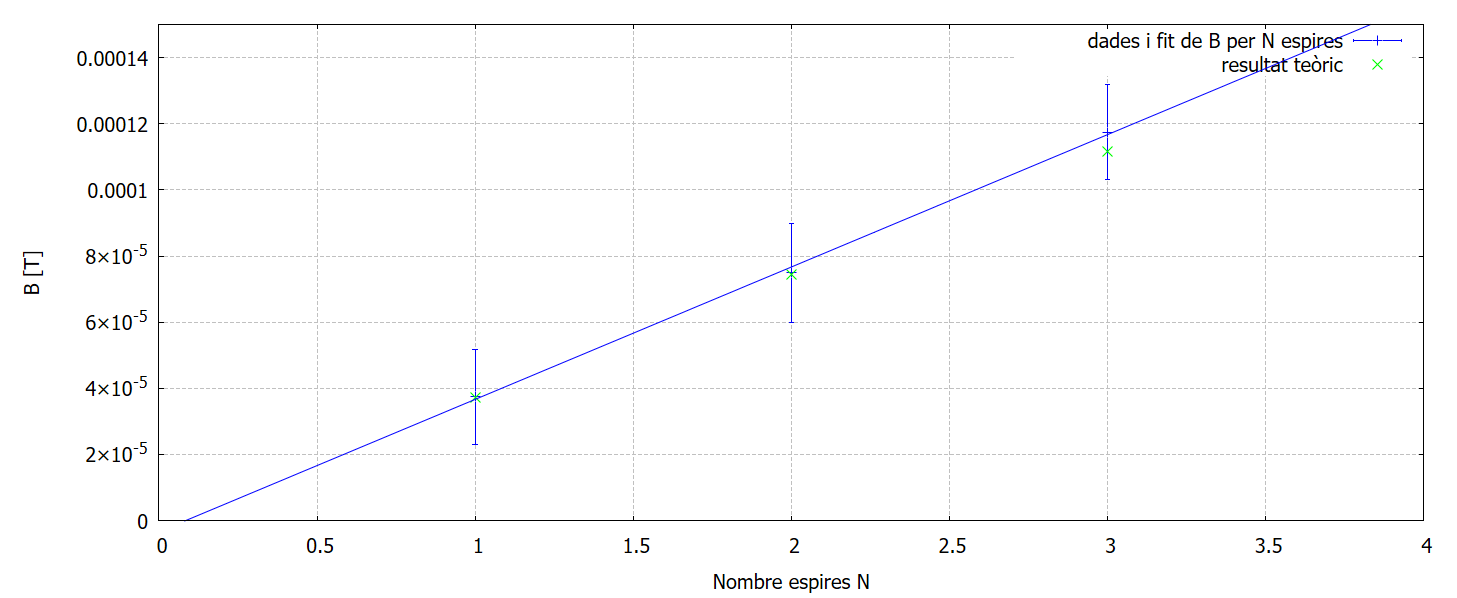
\includegraphics[width=1\linewidth]{BvsN.PNG}
    \caption{Regressió lineal del camp generat $B$ per a un conjunt de $N$ espires en funció del nombre d'espires $N$, comparat amb els valors teòrics.}
    \label{fig:BvsN}
\end{figure}

Mitjançant tots dos mètodes obtenim un valor de la permeabilitat $\mu_0$ que és compatible amb el valor tabulat. Per tant, tots dos mètodes són vàlids per trobar la permeabilitat. Però, donat que la incertesa del segon mètode és menor, considerem que aquest és millor per mesurar la permeabilitat $\mu_0$.


\subsubsection{Mesura del camp de les bobines}\label{subsec: bobines}

\begin{figure}[H]
    \centering
    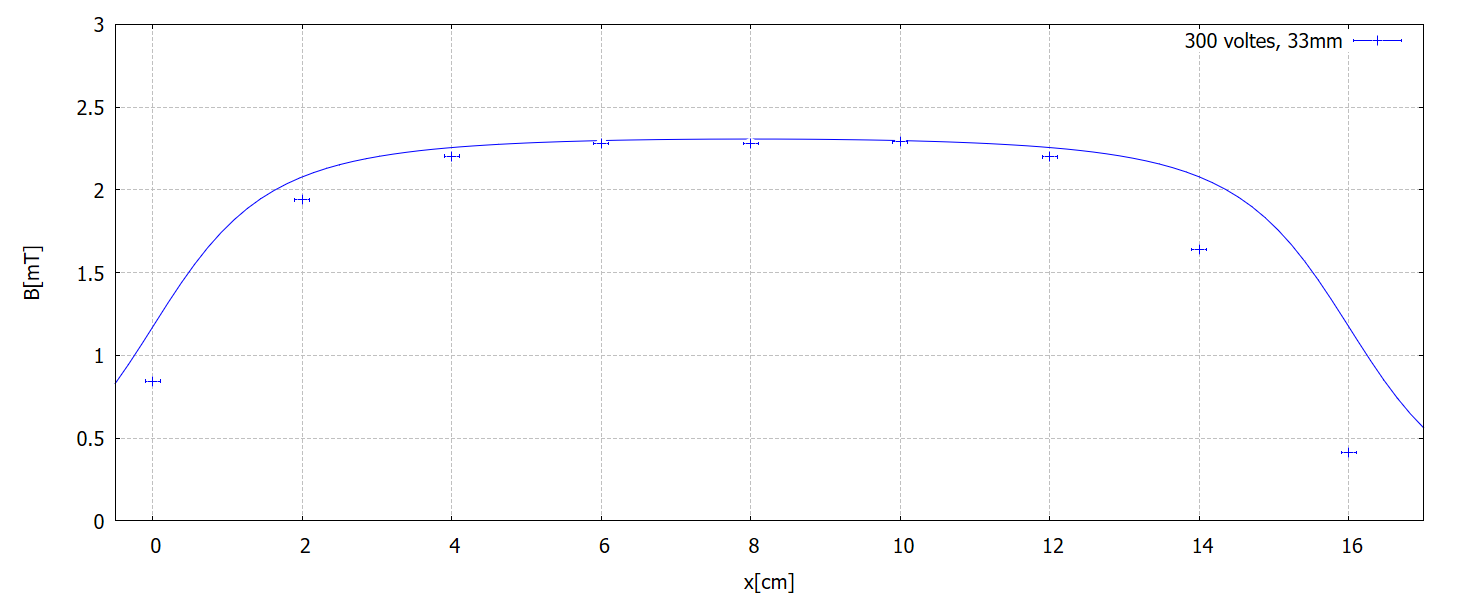
\includegraphics[width=0.75\linewidth]{Bobina 1.PNG}
    \caption{Camp d'inducció $B$ en l'eix d'una bobina (33mm de diàmetre, 16 cm de longitud i 300 voltes) en funció de la posició $x$. Punts experimentals i valor teòric.}
    \label{fig: BvsX_33mm}
\end{figure}

En la Fig. (\ref{fig: BvsX_33mm}) podem veure com el camp d'inducció mesurat proper al centre de la bobina (2,285 $\pm$ 0,014) mT és compatible amb el camp teòric 2,298 mT. Però, els valors mesurats en els extrems de la bobina són significativament més baixos que els valors teòrics.

Aquesta discrepància pot ser deguda a què no vàrem mesurar exactament a l'eix de la bobina. Per saber si aquest és el cas, en la següent secció (\ref{sec: programa}) calcularem numèricament l'expressió del camp $\vec{B}$ a tots els punts de l'espai i observant el comportament de la component $z$ d'aquest (la component que mesura la sonda Hall quan està completament alineada) i el mesurat experimentalment podrem deduir si l'error es deu a una mesura del camp fora de l'eix de la bobina. 

Al comparar el camp d'inducció calculat en la secció (\ref{sec: programa}) amb el camp de la Fig. (\ref{fig: BvsX_33mm}) concloem que una mesura fora de l'eix no pot ser la responsable de la discrepància entre les dades experimentals i la fórmula teòrica.

\begin{figure}[H]
    \centering
    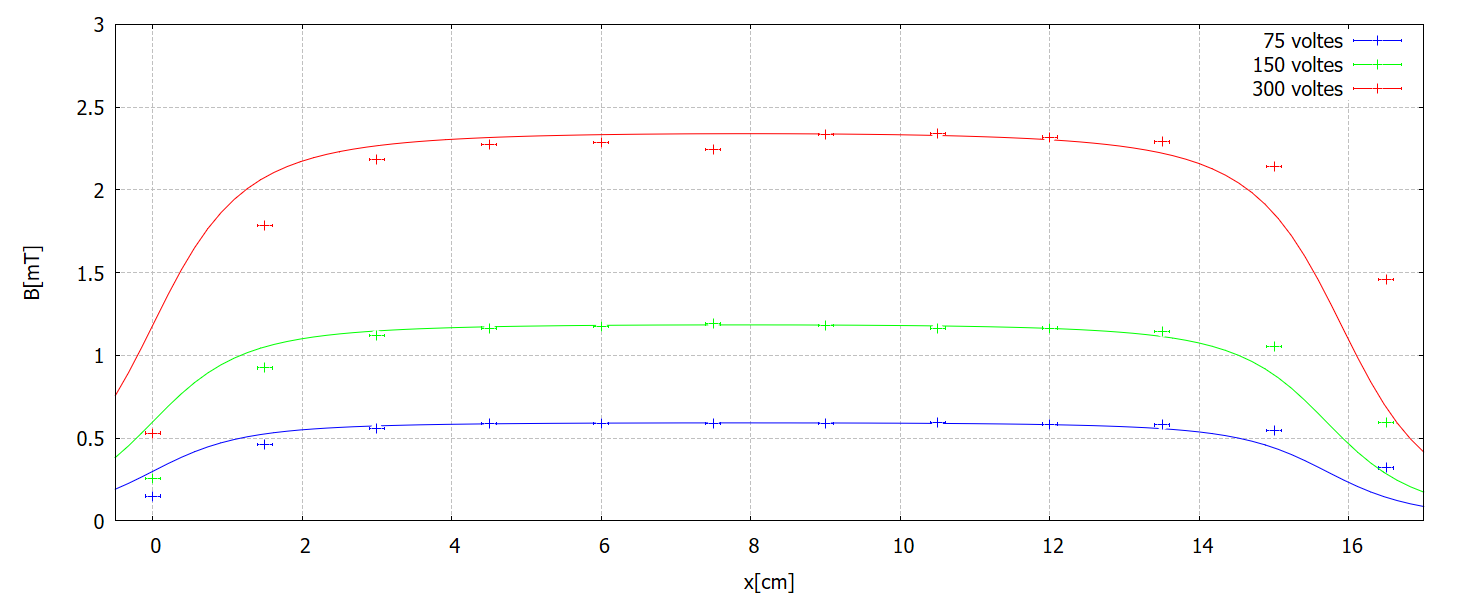
\includegraphics[width=0.75\linewidth]{Bobines 2,3,4.PNG}
    \caption{Camp d'inducció $B$ en l'eix de tres bobines diferents (26mm de diàmetre i 15,8 cm de longitud) en funció de la posició $x$. Punts experimentals i valor teòric.}
    \label{fig: BvsX_26mm}
\end{figure}

En la Fig. (\ref{fig: BvsX_26mm}) podem veure com el camp d'inducció mesurat al voltant dels 6 a 12 cm de les bobines és de (0,590 $\pm$ 0,014) mT, (1,180 $\pm$ 0,014) mT i (2,335 $\pm$ 0,014) mT, és compatible amb el camp teòric 0,591 mT, 1,184 mT i 2,338 mT, respectivament. Però a l'inici, el valor mesurat és significativament menor i al final, significativament més gran. Aquesta desviació respecte del valor teòric pot ser deguda a que la sonda Hall es trobava desplaçada de l'origen al començar a mesurar.

Per tal de comprovar aquesta hipòtesi, hem usat el mètode dels mínims quadrats \footnote{El mètode dels mínims quadrats es troba explicat a l'annex \ref{sec: mínims_quadrats}} per trobar si hi ha un origen on tots els punts experimentals són compatibles. Al aplicar-ho, trobem que per a les tres bobines el nostre origen es trobava 8 mm desplaçat cap a fora. En la Fig. (\ref{fig: Bvsx_26mm}), on es mostren les dades experimentals i teòriques tenint en compte aquest desplaçament de 8 mm, es veu que totes les dades experimentals de les tres bobines són compatibles amb els valors teòrics, excepte el punt a 7,5 cm de la bobina de 300 voltes, que és considerablement menor.

\begin{figure}[H]
    \centering
    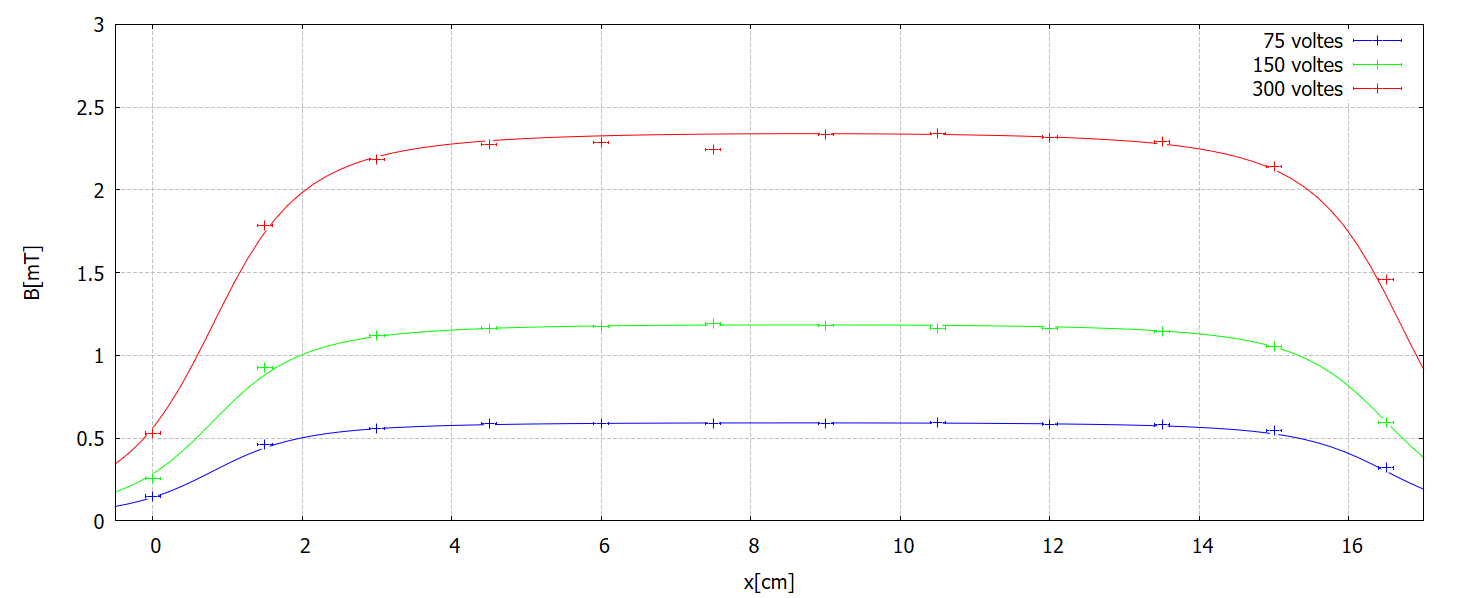
\includegraphics[width=0.75\linewidth]{Bobines 2,3,4 shift 8mm.PNG}
    \caption{Camp d'inducció $B$ en l'eix de tres bobines diferents (26mm de diàmetre i 15,8 cm de longitud) en funció de la posició $x$. Punts experimentals i valor teòric amb l'origen desplaçat.}
    \label{fig: Bvsx_26mm}
\end{figure}

Donat que amb el desplaçament de 8 mm del origen tots els punts, excepte un, són compatibles, confirmem que aquest és el motiu de la desviació entre l'experiment i la teoria. Aquest error es deu a que el nostre mètode per trobar l'origen de la bobina (descrit a la secció \ref{sec: mètode}) és poc exacte. Un mètode més exacte és que el suport de plàstic de les bobines sigui transparent, de manera que l'origen seria el punt on la punta de la sonda es troba just entrant en els cables; les demés posicions se seguirien trobant amb el mètode de la distància relativa, ja que els cables seguirien essent opacs. Un altre mètode més exacte és posar un petit sensor de proximitat a la punta de la sonda i tapar un dels extrems de la bobina; de manera que el sensor mesura la distància de la punta a la tapa i la posició de la punta és aquesta distància menys la distància de la tapa a l'inici dels cables.

D'altra banda, comparant el valor del camp entre elles (bobines de dimensions iguals i diferent nombre de voltes), fent el quocient entre els camps per a cada bobina en cada punt, trobem que el camp per 300 voltes és aproximadament el doble que el de 150 i aquest, alhora, és aproximadament el doble que el de 75 \footnote{Els valors del camp i els quocients es troben a l'annex \ref{PR7_taules_dades_exp} a la Taula \ref{tab: taula Bx}}. Pel que veiem, el camp generat per una bobina és proporcional al nombre de voltes. Confirmant el principi de superposició.


\subsection{Simulació numèrica del camp d'inducció} \label{sec: programa}
Per calcular numèricament el camp d'inducció a tot l'espai hem realitzat un programa de Fortran \footnote{Veure l'annex (\ref{sec: fortran})} que calcula la integral de la fórmula de Biot-Savart (\ref{eq: Biot-Savart}) per a tots els punts del pla $rz$ suposant que la nostra bobina és un conjunt de $N$ espires separades una distància $L/N$ i de radi $R$; com que aquest sistema té simetria de revolució sobre l'eix $z$, podem reduir l'espai tridimensional $x, y, z$ a un espai bidimensional $r, z$ on el camp és constant per $\varphi$ i no té component $\varphi$.

En la Fig. (\ref{fig: Bprog}) es mostra la magnitud i direcció del camp d'inducció $\vec{B}$ de les bobines de la secció anterior (\ref{subsec: bobines}) (Figs. (\ref{fig: BvsX_33mm})). Podem observar com a l'interior de la bobina el camp es manté relativament constant en mòdul i direcció a prop de l'eix i del centre, però segons ens apropem als cables de les bobines, el camp magnètic augmenta en mòdul i, en els extrems, el camp es corba fins a sortir de la bobina perpendicular a aquesta.

\begin{figure}[H]
    \centering
    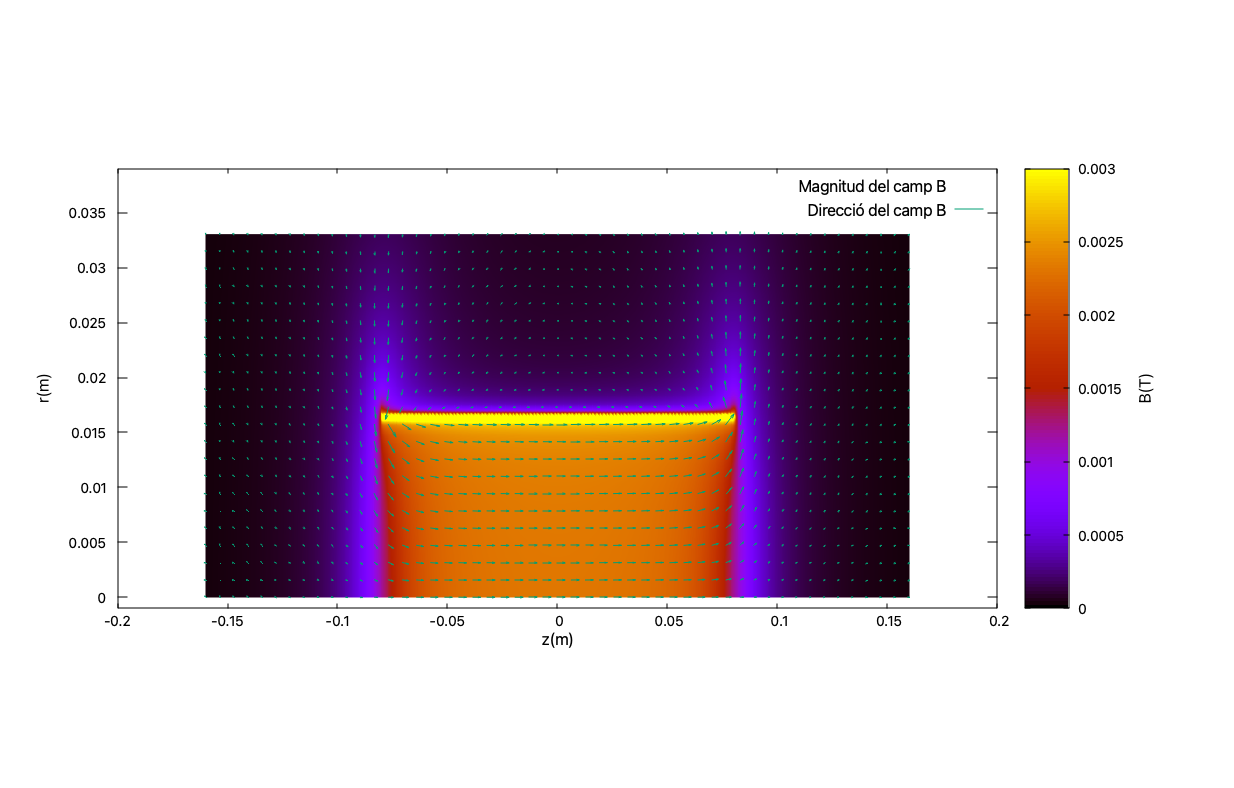
\includegraphics[width=0.75\linewidth]{res.png}
    \caption{Magnitud del camp d'inducció $B$ (mapa de colors) i direcció (vectors verds) generat per una bobina (de 33mm de diàmetre, 300 voltes i 16 cm de longitud per on circula una intensitat de 1 A) en funció de la posició $(z,r)$.}
    \label{fig: Bprog}
\end{figure}

En la Fig. (\ref{fig: zcomp}) es mostra la component $z$ (mesurada per la sonda) del camp $\vec{B}$ de la bobina de 33 mm de diàmetre. Observem que dins de la bobina la component $z$ del camp és constant en $r$ a prop de l'eix, però en apropar-nos suficient als cables, aquesta creix. D'aquesta manera, la hipòtesi formulada a la secció anterior (\ref{subsec: bobines}) per justificar la desviació de les dades experimentals respecte de la fórmula teòrica és incorrecta; ja que aquesta assumia que segons ens allunyàvem de l'eix, el camp havia de disminuir.

\begin{figure}[H]
    \centering
    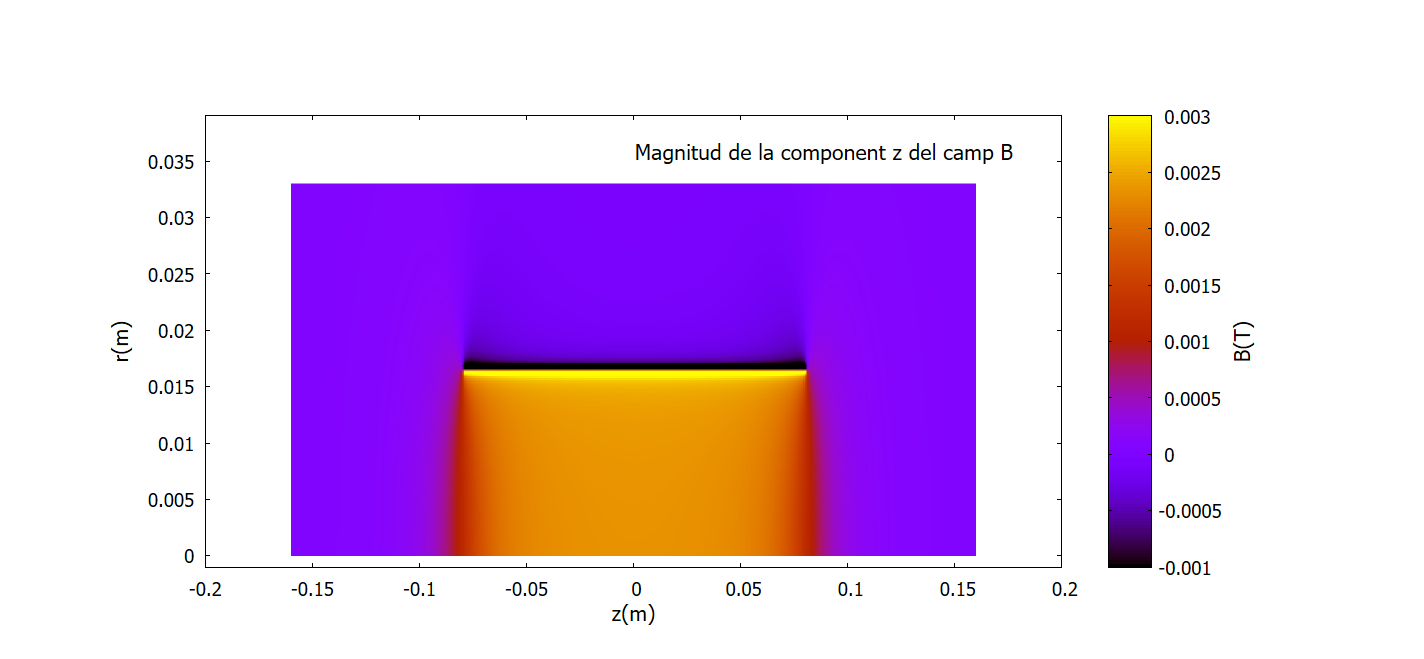
\includegraphics[width=0.75\linewidth]{zcomp.PNG}
    \caption{Magnitud de la component z del camp d'inducció $B$ (mapa de colors) i generat per una bobina (de 33mm de diàmetre, 300 voltes i 16 cm de longitud per on circula una intensitat de 1 A) en funció de la posició $(z,r)$.}
    \label{fig: zcomp}
\end{figure}

\subsection{Conclusions}\label{sec: conclusions}
En aquesta pràctica hem estudiat el camp d'inducció magnètica generat per espires i bobines de diferents radis i nombre de voltes. 

En primer lloc, hem estudiat les dependències amb el radi i el nombre de voltes del camp d'inducció generat per una espira en el seu centre. Obtenint que el camp és proporcional al nombre de voltes i inversament proporcional al radi de l'espira. Concordant amb el resultat teòric obtingut a partir de la llei de Biot-Savart. A més, comparant les dependències obtingudes amb la fórmula experimental hem obtingut dos valors de la permeabilitat magnètica del buit $\mu_0$ = (1,35 $\pm$ 0,55)$\cdot10^{-6}$ N/A$^2$ i $\mu_0$ = (1,35 $\pm$ 0,34)$\cdot10^{-6}$ N/A$^2$, tots dos compatibles amb el valor tabulat de $\mu_0 =$  1,25664 $\cdot 10^{-6}$ N/A$^2$.

En segon lloc, hem estudiat el camp generat per diferents bobines al llarg del seu eix. Obtenint perfils del camp d'inducció que en el centre són compatibles amb el resultat teòric, però que en els extrems no ho són. Hem pogut deduir que aquests errors es deuen a una metodologia inexacta. A més, comparant els perfils obtinguts per tres bobines de la mateixa geometria però amb diferent nombre de voltes, observem que els camps d'inducció són proporcionals al nombre de voltes; resultat compatible amb el principi de superposició.



\newpage

\appendix
\section{Annex}


\subsection{Resultats experimentals}\label{taules_dades_exp}
\subsubsection{Dades experimentals Pràctica 1}
\begin{table}[ht]
    \centering
    \caption{Mesures de $\Delta l$, $\Delta r$ i $\Delta V$ amb inserteses}
    \begin{tabular}{ccc}
        \hline
        $\Delta l$ (m) & $\Delta r$ (m) & $\Delta V$ (V) \\
        \hline
        $0.009 \pm 0.001$ & $0.012 \pm 0.001$ & $1.5 \pm 0.1$ \\
        $0.007 \pm 0.001$ & $0.026 \pm 0.001$ & $1.5 \pm 0.1$ \\
        $0.011 \pm 0.001$ & $0.036 \pm 0.001$ & $1.5 \pm 0.1$ \\
        $0.011 \pm 0.001$ & $0.047 \pm 0.001$ & $1.5 \pm 0.1$ \\
        $0.009 \pm 0.001$ & $0.054 \pm 0.001$ & $1.5 \pm 0.1$ \\
        $0.001 \pm 0.001$ & $0.055 \pm 0.001$ & $1.5 \pm 0.1$ \\
        $0.009 \pm 0.001$ & $0.043 \pm 0.001$ & $1.5 \pm 0.1$ \\
        $0.011 \pm 0.001$ & $0.030 \pm 0.001$ & $1.5 \pm 0.1$ \\
        $0.006 \pm 0.001$ & $0.019 \pm 0.001$ & $1.5 \pm 0.1$ \\
        $0.008 \pm 0.001$ & $0.015 \pm 0.001$ & $1.5 \pm 0.1$ \\
        $0.007 \pm 0.001$ & $0.007 \pm 0.001$ & $1.5 \pm 0.1$ \\
        $0.005 \pm 0.001$ & $0.005 \pm 0.001$ & $1.5 \pm 0.1$ \\
        $0.010 \pm 0.001$ & $0.003 \pm 0.001$ & $1.5 \pm 0.1$ \\
        $0.010 \pm 0.001$ & $0.005 \pm 0.001$ & $1.5 \pm 0.1$ \\
        $0.009 \pm 0.001$ & $0.004 \pm 0.001$ & $1.5 \pm 0.1$ \\
        $0.010 \pm 0.001$ & $0.004 \pm 0.001$ & $1.5 \pm 0.1$ \\
        $0.010 \pm 0.001$ & $0.004 \pm 0.001$ & $1.5 \pm 0.1$ \\
        $0.010 \pm 0.001$ & $0.005 \pm 0.001$ & $1.5 \pm 0.1$ \\
        $0.008 \pm 0.001$ & $0.005 \pm 0.001$ & $1.5 \pm 0.1$ \\
        $0.015 \pm 0.001$ & $0.004 \pm 0.001$ & $1.5 \pm 0.1$ \\
        \hline
    \end{tabular}
    
    \label{tab:mesures}
\end{table}


\subsubsection{Resultats experimentals Pràctica 2}\label{PR2_taules_dades_exp}

%TAULES DADES EXPERIMENTALS

\begin{table}[h!]
\centering
\caption{Taula d'intensitats de corrent (A) en funció de la massa (mg)}
\begin{tabular}{|c|c|c|c|c|c|}
\hline
\textbf{Massa (mg)} & \textbf{5 $\pm$ 0.4 } & \textbf{10 $\pm$ 0.4 } & \textbf{15 $\pm$ 0.4} & \textbf{20 $\pm$ 0.4 } & \textbf{25 $\pm$ 0.4 } \\
\hline
 & 2.71 $\pm$ 0.01 & 4.38 $\pm$ 0.01 & 5.21 $\pm$ 0.01 & 6.23 $\pm$ 0.01 & 7.70 $\pm$ 0.01 \\
\textbf{I (A)} & 2.66 $\pm$ 0.01 & 4.2 $\pm$ 0.012 & 5.13 $\pm$ 0.01 & 6.44 $\pm$ 0.01 & 7.58 $\pm$ 0.01 \\
 & 2.71 $\pm$ 0.01 & 4.10 $\pm$ 0.01 & 5.47 $\pm$ 0.01 & 6.38 $\pm$ 0.01 & 7.81 $\pm$ 0.01 \\
\hline
\end{tabular}
\end{table}

\begin{table}[H]
\centering
\caption{Taula d'angles ($\theta$) en funció de la massa (mg)}
\begin{tabular}{|c|c|}
\hline
\textbf{Massa (mg)} & \textbf{Angle ($\theta$)} \\
\hline
5 $\pm$ 0.4   & 17 $\pm$ 1 \\
10 $\pm$ 0.4  & 31 $\pm$ 1 \\
15 $\pm$ 0.4  & 45 $\pm$ 1 \\
20 $\pm$ 0.4  & 58 $\pm$ 1 \\
25 $\pm$ 0.4  & 69 $\pm$ 1 \\
\hline
\end{tabular}
\end{table}

\begin{table}[H]
\centering
\caption{Taula d'angles ($\theta$) en funció de la distància de separació entre fils (mm)}
\begin{tabular}{|c|c|c|c|c|}
\hline
\textbf{Distància separació (mm)} & \textbf{4 $\pm$ 1} & \textbf{6 $\pm$ 1} & \textbf{8 $\pm$ 1} & \textbf{10 $\pm$ 1} \\
\hline
\textbf{Angle ($\theta$}) & 64 $\pm$ 1  & 47  $\pm$ 1 & 41  $\pm$ 1 & 30  $\pm$ 1 \\
   & 60  $\pm$ 1 & 48  $\pm$ 1 & 39  $\pm$ 1 & 31  $\pm$ 1 \\
\hline
\end{tabular}
\end{table}

\subsubsection{Resultats experimentals Pràctica 6}
\begin{figure}[h]
    \centering
    \begin{minipage}{0.45\textwidth}
        \centering
        \captionof{table}{Resultats experimentals dels radis de la trajectòria per cada valor de potencial d'acceleració.}
        \begin{tabular}{|c|c|}
            \hline
            Va (V)	&	R (m)	\\\hline
            (2000 ± 200)	&	(0.0880± 0.0077)	\\\hline
            (3000 ± 200)	&	(0.107± 0.011)	\\\hline
            (4000 ± 200)	&	(0.120± 0.014)	\\\hline
            (5000 ± 200)	&	(0.128 ± 0.015)	\\\hline
            
        \end{tabular}
        
        \label{tab:RvsVa}
    \end{minipage}
    \hfill
    \begin{minipage}{0.45\textwidth} 
        \centering
        \captionof{table}{Resultats experimentals dels radis de la trajectòria per cada valor d'intensitat de corrent.}
        \begin{tabular}{|c|c|}
            \hline
            I(A)	&	R (m)	\\\hline
            (0,800 ± 0,010)	&	(0,0494 ± 0,0037)	\\\hline
            (0,700 ± 0,010)	&	(0,0570± 0,0048)	\\\hline
            (0,600 ± 0,010)	&	(0,0685 ± 0,0051)	\\\hline
            (0,500 ± 0,010)	&	(0,0808± 0,0082)	\\\hline
            (0,400 ± 0,010)	&	(0,0983 ± 0,0089)	\\\hline
            (0,300 ± 0,010)	&	(0,1298 ± 0,016)	\\\hline
            (0,200 ± 0,010)	&	(0,201 ± 0,034)	\\\hline
            (0,100 ± 0,010)	&	(0,26 ± 0,10)	\\\hline
            
        \end{tabular}
        
        \label{tab:RvsI}
    \end{minipage}
\end{figure}

\begin{table}[h!]
    \centering
    \caption{Resultats experimentals de la trajectòria amb valor de potencial (fixa camp $\vec{E}$) entre les plaques constant.}
    \begin{tabular}{|c|c|c|}
        \hline
        \textbf{Vp (kV)} & \textbf{x (cm)} & \textbf{y (cm)} \\
        \hline
         & 1.00 $\pm$ 0.10 & 0.00 $\pm$ 0.10 \\
         & 2.00 $\pm$ 0.10 & 0.02 $\pm$ 0.10 \\
        0.85 $\pm$ 0.20 & 3.00 $\pm$ 0.10 & 0.10 $\pm$ 0.10 \\
         & 4.00 $\pm$ 0.10 & 0.21 $\pm$ 0.10 \\
         & 5.00 $\pm$ 0.10 & 0.32 $\pm$ 0.10 \\
        \hline
    \end{tabular}
    
\end{table}

\begin{table}[h!]
    \centering
    \caption{Resultats experimentals de la trajectòria amb valors d'intensitat de corrent (fixa camp $\vec{B}$) i potencial entre les plaques (fixa camp $\vec{E}$) constants.}
    \begin{tabular}{|c|c|c|c|}
        \hline
        \textbf{Vp (kV)} & \textbf{I (A)} & \textbf{x (cm)} & \textbf{y (cm)} \\
        \hline
         &  & 2.00 $\pm$ 0.10 & 0.01 $\pm$ 0.10 \\
         &  & 3.00 $\pm$ 0.10 & 0.23 $\pm$ 0.10 \\
        0.85 $\pm$ 0.20 & 0.10 $\pm$ 0.01 & 4.00 $\pm$ 0.10 & 0.35 $\pm$ 0.10 \\
         &  & 5.00 $\pm$ 0.10 & 0.47 $\pm$ 0.10 \\
         &  & 6.00 $\pm$ 0.10 & 0.65 $\pm$ 0.10 \\
        \hline
    \end{tabular}
    
\end{table}

\subsubsection{Resultats experimentals Pràctica 7} \label{PR7_taules_dades_exp}

\begin{table}[H]
    \centering
        \begin{tabular}{|c|c|c|c|c|c|}
            \hline
            x(cm)	&	B$_{75}(mT)$   & B$_{150}$ (mT)    & B$_{300}$ (mT) &	 B$_{150}$/B$_{75}$ & B$_{300}$/B$_{150}$ \\\hline
            0.0 ± 0.1 	&	0.150 ± 0.014   & 0.255 ± 0.014     & 0.530 ± 0.014     & 1.7  & 2.1
	    \\\hline
            1.5 ± 0.1	&	0.460 ± 0.014   & 0.925 ± 0.014     & 1.785 ± 0.014     & 2.0  & 1.9
	\\\hline
            3.0 ± 0.1	&	0.560 ± 0.014   & 1.120 ± 0.014     & 2.185 ± 0.014     & 2.0  & 2.0
	\\\hline
            4.5 ± 0.1	&	0.590 ± 0.014   & 1.165 ± 0.014     & 2.275 ± 0.014     & 2.0  & 2.0
	\\\hline
            6.0 ± 0.1	&	0.590 ± 0.014   & 1.175 ± 0.014     & 2.285 ± 0.014     & 2.0  & 1.9
	\\\hline
            7.5 ± 0.1	&	0.590 ± 0.014   & 1.190 ± 0.014     & 2.245 ± 0.014     & 2.0  & 1.9
	\\\hline
            9.0 ± 0.1	&	0.590 ± 0.014   & 1.180 ± 0.014     & 2.335 ± 0.014     & 2.0  & 2.0
	\\\hline
            10.5 ± 0.1	&	0.595 ± 0.014   & 1.165 ± 0.014     & 2.340 ± 0.014     & 2.0  & 2.0
	\\\hline
            12.0 ± 0.1  &   0.585 ± 0.014   & 1.165 ± 0.014     & 2.320 ± 0.014     & 2.0  & 2.0
        \\\hline
            13.5 ± 0.1  &   0.580 ± 0.014   & 1.145 ± 0.014     & 2.290 ± 0.014     & 2.0  & 2.0
        \\\hline
            15.0 ± 0.1  &   0.545 ± 0.014   & 1.055 ± 0.014     & 2.140 ± 0.014     & 1.9  & 2.0
        \\\hline
            16.5 ± 0.1  &   0.320 ± 0.014   & 0.595 ± 0.014     & 1.460 ± 0.014     & 1.9  & 2.5
        \\\hline
        \end{tabular}
    \caption{Resultats experimentals del camp d'inducció $B$ en funció de la posició $x$ de tres bobines de 75, 150 i 300 voltes, mesurat al eix.}
    \label{tab: taula Bx}
\end{table}


\subsection{Imatges} \label{sec: imatges}
\subsubsection{Imatges del muntatge experimental de la pràctica 1}\label{fotos}
\begin{figure}[H]
    \centering

    \begin{subcaptionbox}{Condensador\label{fig:img1}}[0.3\textwidth]
        {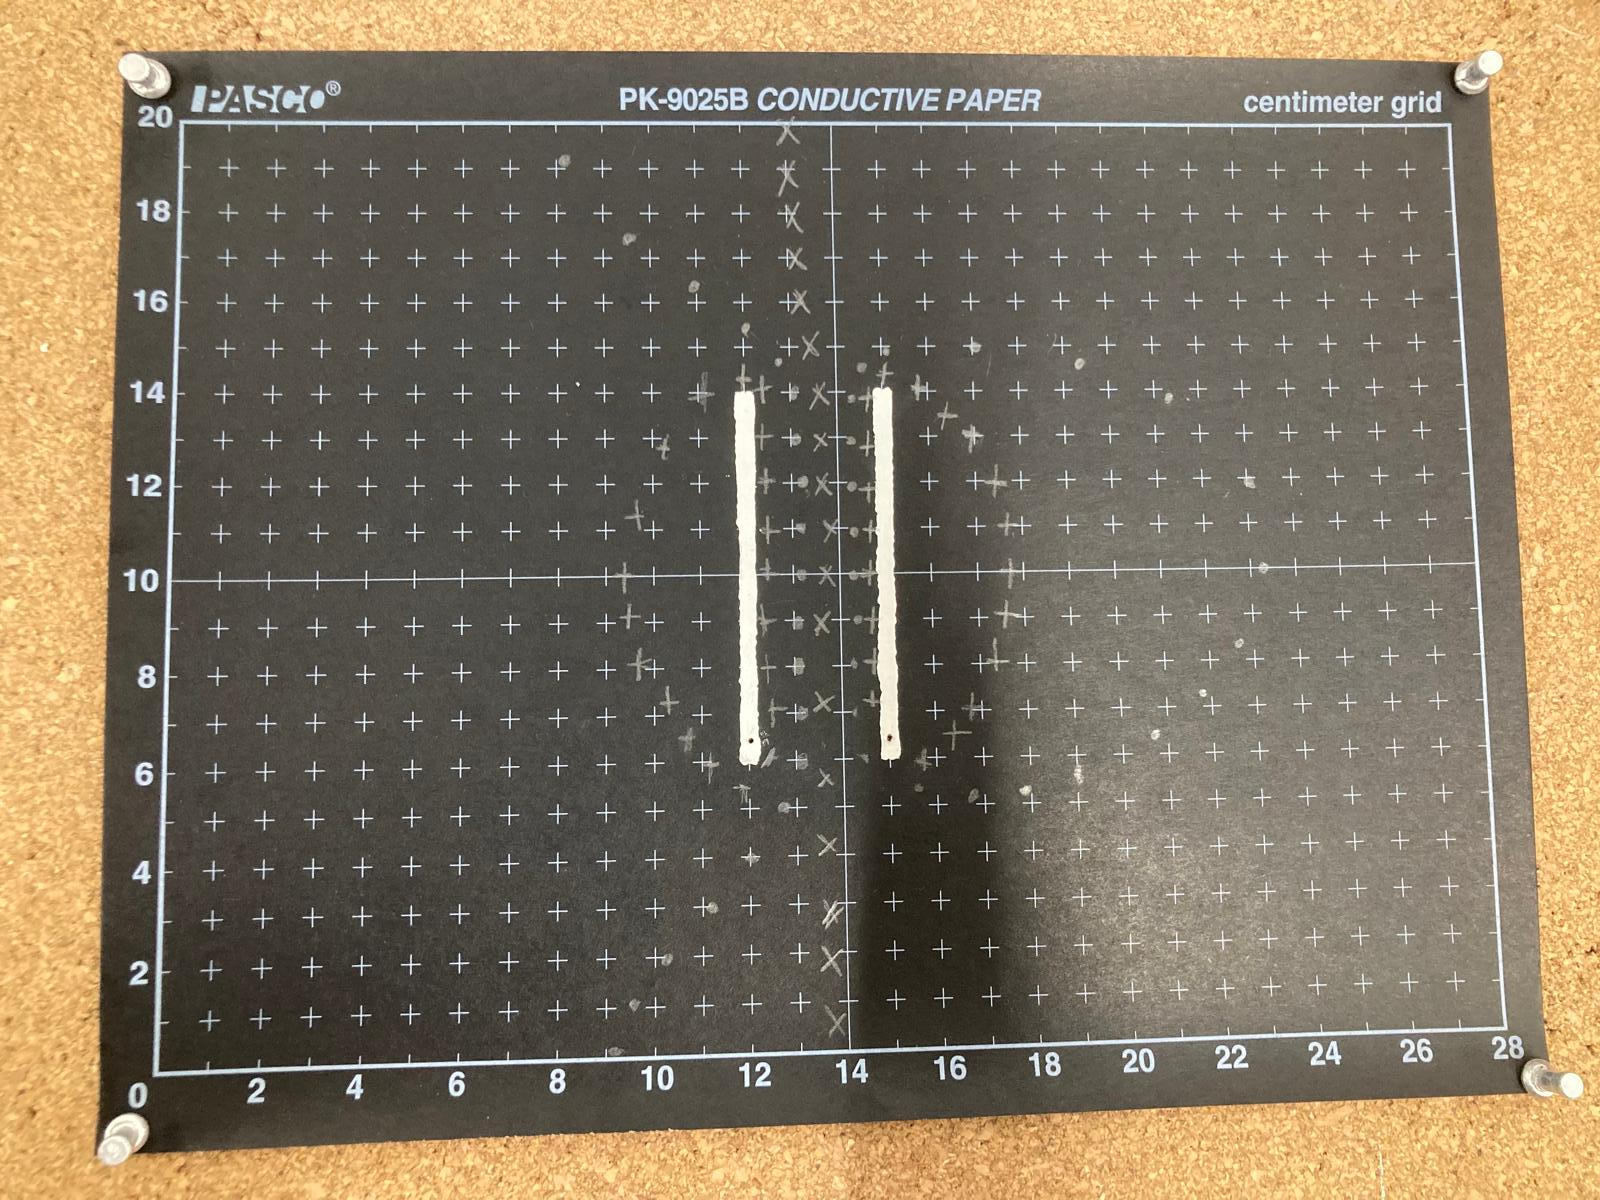
\includegraphics[width=\linewidth]{imatge1.jpg}}
    \end{subcaptionbox}
    \hfill
    \begin{subcaptionbox}{Fils inifnits\label{fig:img2}}[0.3\textwidth]
        {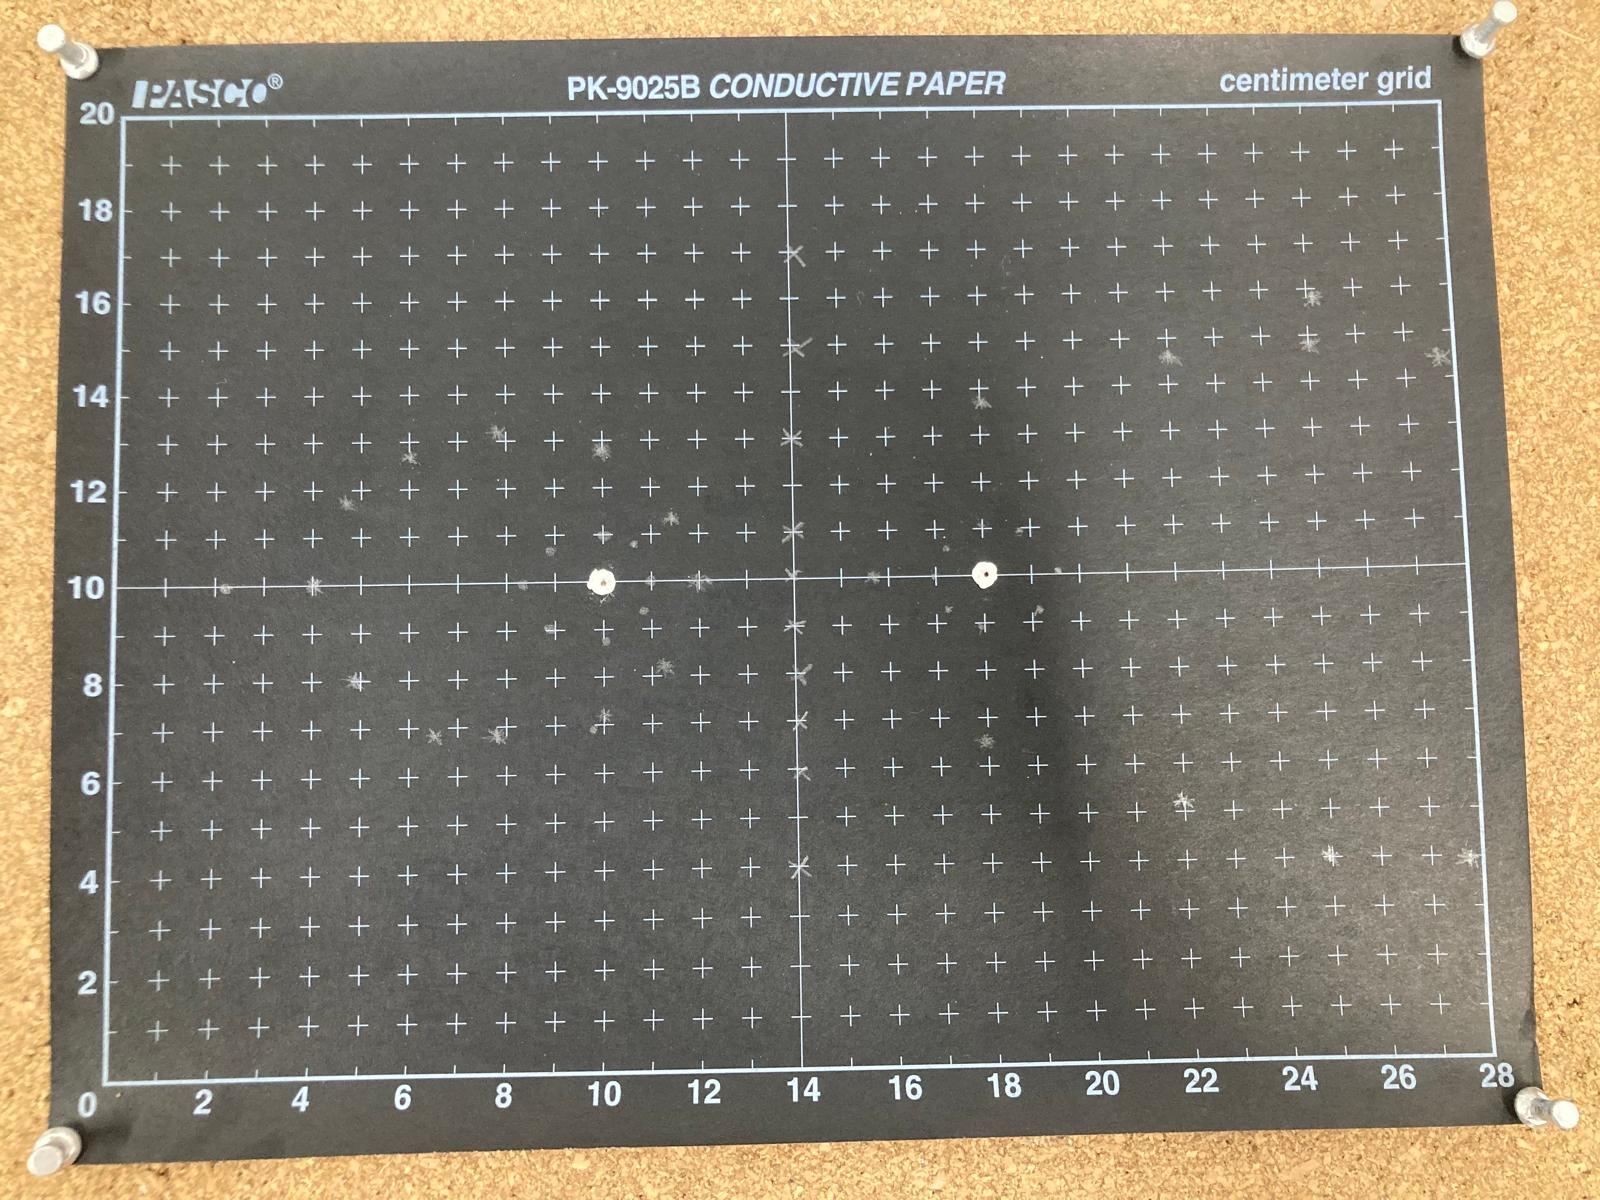
\includegraphics[width=\linewidth]{imatge2.jpg}}
    \end{subcaptionbox}
    \hfill
    \begin{subcaptionbox}{Configuració lliure\label{fig:img3}}[0.3\textwidth]
        {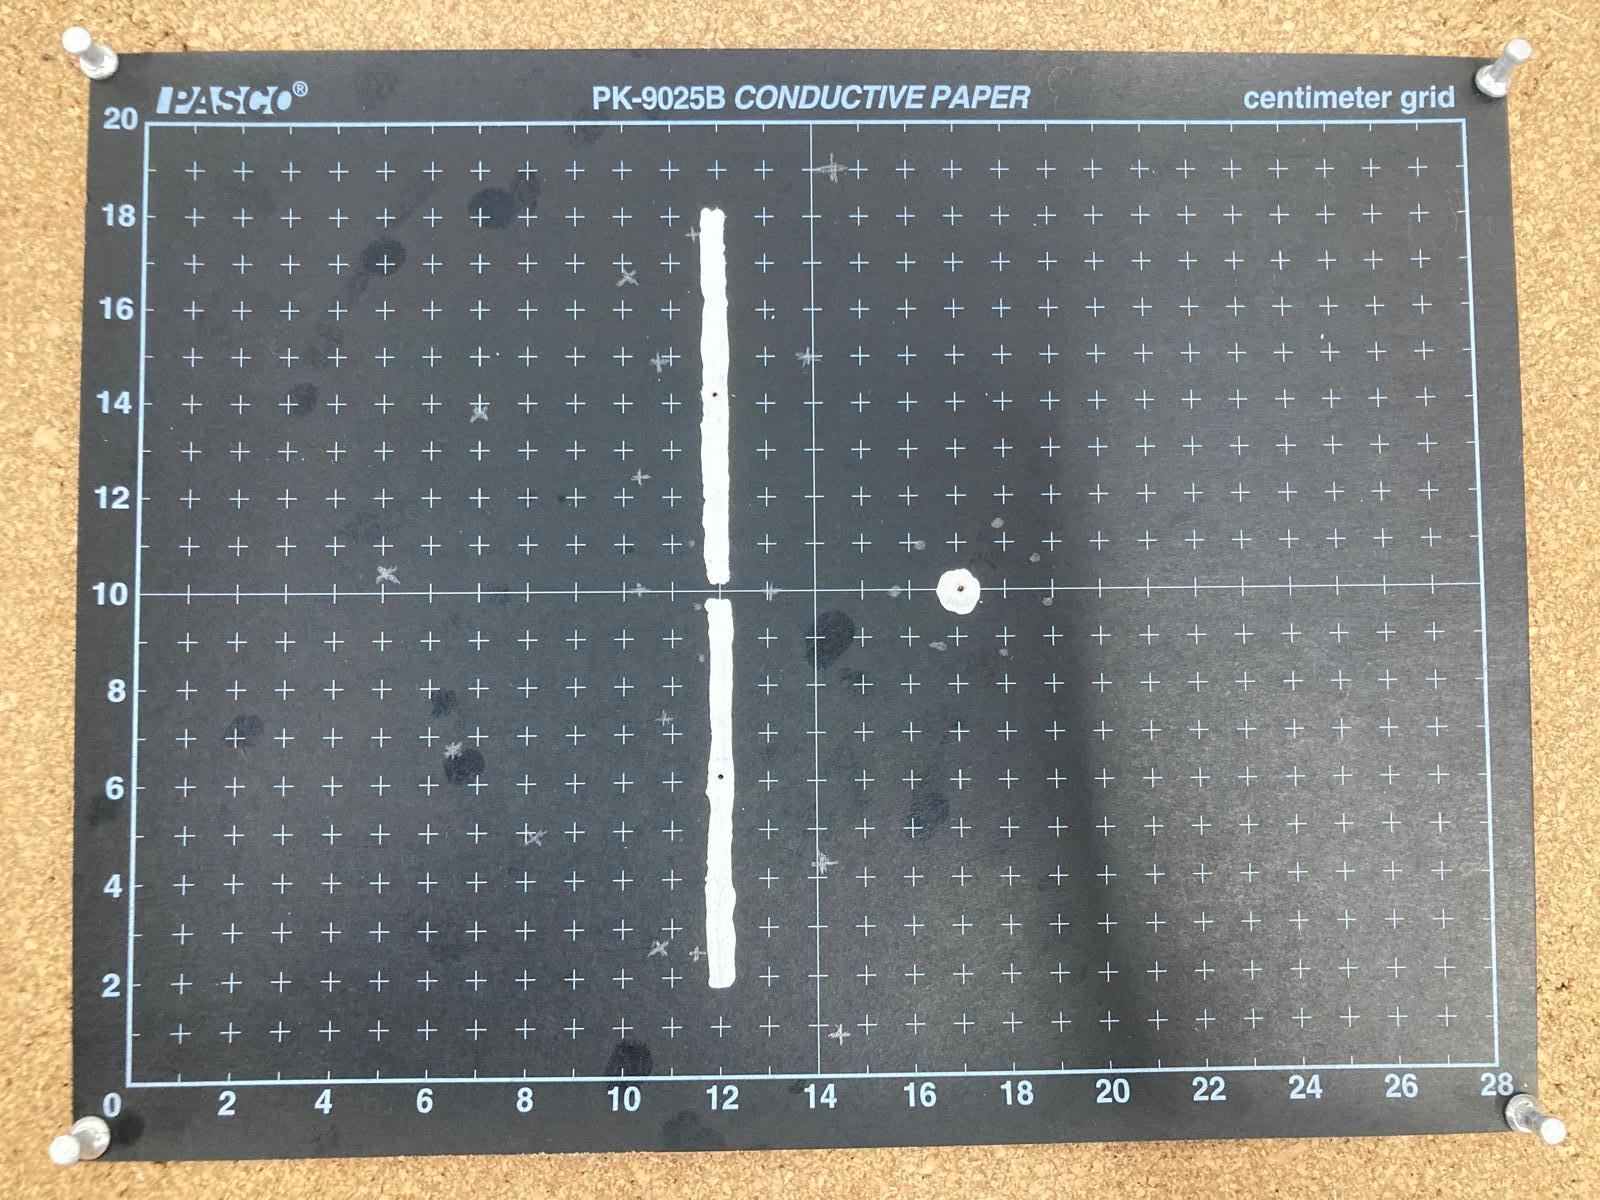
\includegraphics[width=\linewidth]{imatge3.jpg}}
    \end{subcaptionbox}

    \caption{Muntatge experimental de les tres distribucions de conductors.}
    \label{fig:figura3}
\end{figure}
\subsubsection{imatges pràctica 6}
\begin{figure}[H]
    \centering
    \begin{minipage}{0.38\textwidth}
        \centering
        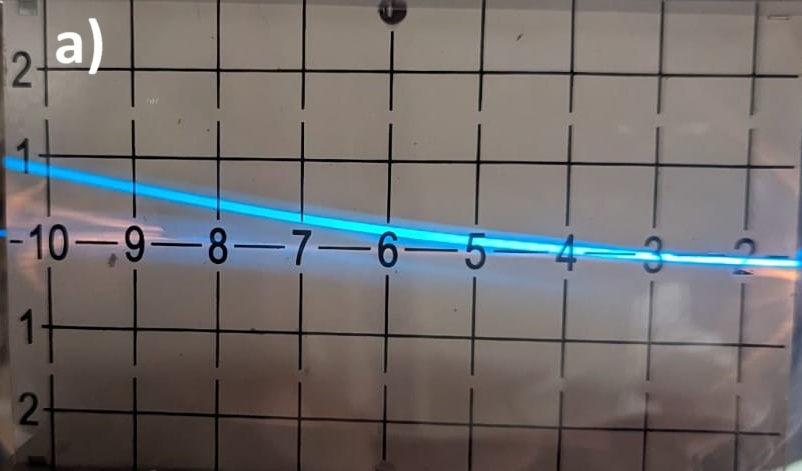
\includegraphics[width=\textwidth]{1kV.jpg}
    \end{minipage}
    \begin{minipage}{0.38\textwidth}
        \centering
        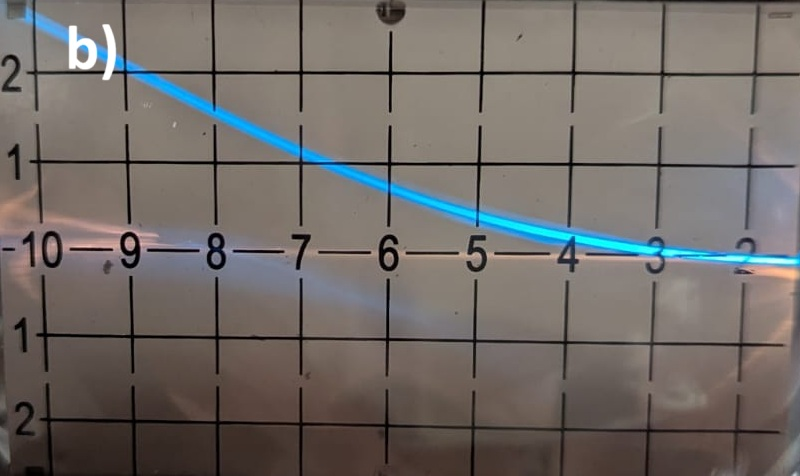
\includegraphics[width=\textwidth]{2kV.jpg}
    \end{minipage}
    \begin{minipage}{0.38\textwidth}
        \centering
        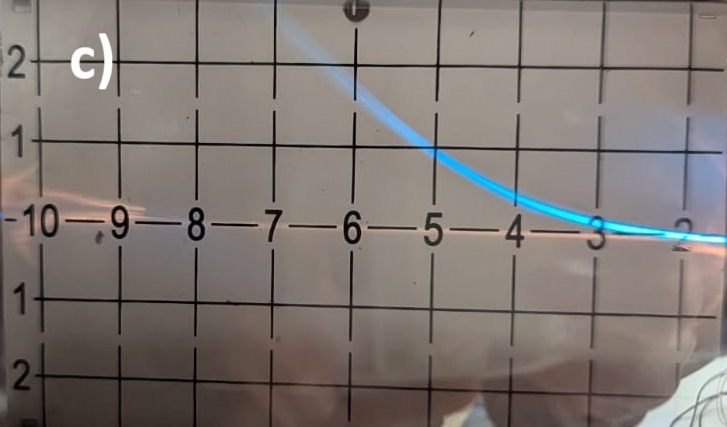
\includegraphics[width=\textwidth]{3kV.jpg}
    \end{minipage}
    \begin{minipage}{0.38\textwidth}
        \centering
        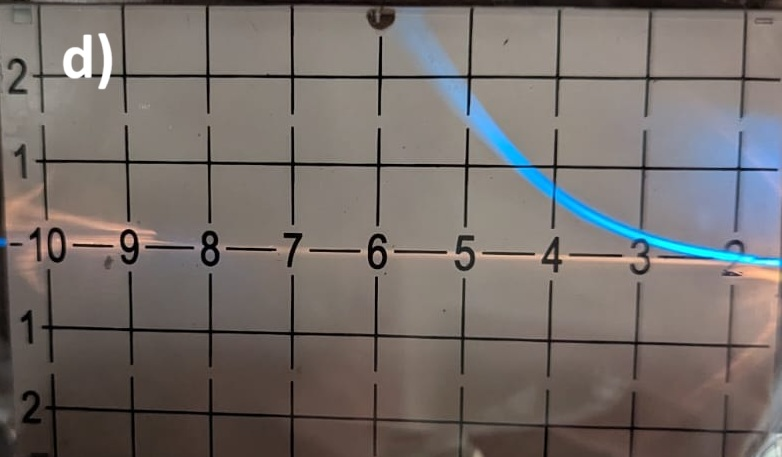
\includegraphics[width=\textwidth]{4kV.jpg}
    \end{minipage}
    \caption{Desviació del raigs en presència del camp elèctric generat per les plàques. (a) 1kV, (b) 2kV, (c) 3kV, (d) 4kV}
    \label{fig: Desv E}
\end{figure}
\subsection{Càlcul d'incerteses}
\underline{Incertesa estadística de la mitja d'un conjunt de mesures:} La fórmula per trobar l'incertesa estadística d'un conjunt de mesures és:
\begin{equation} \label{eq: incertesa estadística}
    u^2 = \frac{1}{N(N-1)} \sum_{i=1}^{N} (x_i - <x>)^2
\end{equation}
on ${x_i}$ són les variables mesurades, $<x>$ la seva mitjana i $N$ el nombre de variables mesurades.

\underline{Incertesa total:} Per obtenir l'incertesa total d'una mesura a partir de les incerteses estadístiques i instrumentals usem:
\begin{equation} \label{eq: incertesa total}
    u_{Total}^2 = u_{ins}^2+u_{est}^2
\end{equation}

\underline{Propagació d'errors:}  Per trobar les incerteses de magnituds dependents d'altres magnituds mesurables hem usat l'equació de propagació d'incerteses
\begin{equation} \label{eq: propagació d'errors}
    u_{y}^2=\sum_{i=1}^{N}(\frac{\partial y}{\partial x_i})^2u_{x_i}^2
\end{equation}
on y és la magnitud dependent i ${x_i}$ les variables mesurables.

\subsubsection{Càlcul d'incerteses Pràctica 1}
\begin{equation}
    u_{Q/L} = \varepsilon \sqrt{
        \left( \sum_i \frac{\Delta l_i}{\Delta r_i} \right)^2 u^2_{\Delta \phi_i} +
        \left( \sum_i \frac{\Delta \phi_i}{\Delta r_i} \right)^2 u^2_{\Delta l_i} +
        \left( \sum_i \frac{\Delta \phi_i \Delta l_i}{\Delta r_i^2} \right)^2 u^2_{\Delta r_i}}
        \label{eq: ins_q}
\end{equation}


\begin{equation}
    u_{C/L} = \sqrt{
        \left( \frac{1}{\Delta V} \right)^2 u^2_{Q/L} +
        \left( \frac{Q/L}{\Delta V^2} \right)^2 u^2_{\Delta V}}
    \label{eq: ins_c}
\end{equation}

\begin{equation}
    u_{(C/L)_t} = \varepsilon \sqrt{
    \left( \frac{1}{d} \right)^2 u^2_l +
    \left( \frac{l}{d^2} \right)^2 u^2_d}
    \label{eq: ins_ct}
\end{equation}

\subsubsection{Càlcul d'incerteses pràctica 2}\label{sec: PR2_calcul_incerteses}

L'incertesa de $\mu_0$ a partir de les dades de regressió \ref{fig: PR2_regr_I2vsF}:
\begin{equation}
    u_{\mu_0}^2 = \left(\frac{2\pi r}{m^2L}\right)^2u_m^2 + \left(\frac{2\pi r}{mL^2}\right)^2u_I^2 + \left(\frac{2\pi}{mL}\right)^2u_r^2
\end{equation}

L'incertesa de $F$ per obtenir les dades de regressió \ref{fig: PR2_regr_Fvstheta}:
\begin{equation}
    u_{F}^2 = k^2u_{theta}^2 + \theta^2u_{k}^2
\end{equation}

L'incertesa de $\mu_0$ a partir de les dades de regressió \ref{fig: PR2_regr_thetavsr}:
\begin{equation}
    u_{\mu_0}^2 = \left(\frac{2\pi k}{LI^2}\right)^2u_m^2 + \left(\frac{2\pi m}{LI^2}\right)^2u_k^2 + \left(\frac{2\pi km}{L^2I^2}\right)^2u_L^2 + \left(\frac{4\pi km}{LI^3}\right)^2u_L^2
\end{equation}

L'incertesa de $B_{t_{norm}}$ a partir de l'Eq. \eqref{eq: PR2_Btnorm}:
\begin{equation}
    u_{\mu_0}^2 = \left(\frac{2\pi r}{m^2L}\right)^2u_m^2 + \left(\frac{2\pi r}{mL^2}\right)^2u_I^2 + \left(\frac{2\pi}{mL}\right)^2u_r^2
\end{equation}

\subsubsection{Càlcul d'incerteses Pràctica 6}

Per a aquest estudi, s’han considerat diverses fonts d’incertesa relacionades amb els valors mesurats. Els potencials elèctrics \( V_a \) i \( V_p \) tenen una incertesa assignada de \( 0{,}2~\text{kV} \) cadascun. La mesura de la intensitat del corrent elèctric a la bobina presenta una incertesa de \( 0{,}01~\text{A} \), mentre que la distància entre les plaques, representada per \( d \), es determina amb una precisió de \( \pm 1~\text{mm} \).

El càlcul de la incertesa sobre la constant \( k \), que reflecteix els efectes marginals del camp elèctric entre plaques paral·leles, es basa en l’equació següent:

\begin{equation}
    u_k = \sqrt{
        \left( \frac{4 V_a A}{V_p} u_d \right)^2 +
        \left( \frac{4 d A}{V_p} u_{V_a} \right)^2 +
        \left( \frac{4 d V_a}{V_p} u_A \right)^2 +
        \left( \frac{-4 d V_a A}{V_p^2} u_{V_p} \right)^2
    }
    \label{eq:k}
\end{equation}

A continuació, es determina la incertesa en el càlcul de la relació \( q/m \) (càrrega respecte a la massa), utilitzant les dades obtingudes de l’estudi de la desviació provocada per un camp magnètic. Aquesta es calcula mitjançant:

\begin{equation}
    u_{q/m} = \sqrt{
        \left( \frac{2}{K^2 I^2 R^2} u_{V_a} \right)^2 +
        \left( \frac{-4 V_a}{K^2 R^2 I^3} u_I \right)^2 +
        \left( \frac{-4 V_a}{K^2 I^2 R^3} u_R \right)^2
    }
    \label{eq:qm1}
\end{equation}

Per obtenir un valor fiable de \( q/m \), es fa una mitjana a partir de diverses mesures. Si designem \( (q/m)_i \) com el resultat de la \( i \)-èsima mesura, i se’n realitzen \( n \), la incertesa global associada al valor mitjà s’expressa com:

\begin{equation}
    u_{\langle q/m \rangle} = \frac{1}{n} \sqrt{ \sum_{i=1}^n u_{(q/m)_i}^2 }
    \label{eq:mean}
\end{equation}

En el cas de mesures amb \( V_a \) fix i intensitat variable, es van realitzar vuit registres (\( n = 8 \)), mentre que amb intensitat constant i \( V_a \) variable es van fer quatre (\( n = 4 \)).

Finalment, es torna a calcular la relació \( q/m \), ara a partir de les dades de desviació electromagnètica. En aquest pas s’inclou també la incertesa associada a la constant \( k \), segons el valor obtingut prèviament:

\begin{equation}
    u_{q/m} = \sqrt{
        \left( \frac{V_p}{d K^2 I^2 R} u_k \right)^2 +
        \left( \frac{k}{d K^2 I^2 R} u_{V_p} \right)^2 +
        \left( \frac{-k V_p}{K^2 I^2 R d^2} u_d \right)^2 +
        \left( \frac{-2 k V_p}{d I^3 R K^3} u_I \right)^2 +
        \left( \frac{-k V_p}{d K^2 I^2 R^2} u_R \right)^2
    }
    \label{eq:qm2}
\end{equation}

\subsubsection{Càlcul d'incerteses Pràctica 7}\label{sec: incerteses}


\underline{Incertesa instrumental Pràcitca 7:}
Com a incertesa de qualsevol longitud mesurada hem agafat $u_d = 10^{-3}m$, que és la distància mínima que les regles podien mesurar.
Per les incerteses de les intensitats i camps d'inducció no hem agafat el valor mínim que podien mesurar l'amperímetre i teslametre perquè tots dos no donaven un valor fix; hem agafat el rang de valors on oscil·lava la mesura $u_I = 10^{-3}A$ i $u_B = 2 \cdot 10^{-5}T$.

\underline{Incertesa equacions Pràctica 7:}

L'incertesa de l'Eq (\ref{eq: B_semidif}) :
\begin{equation}
    u_{B_{semidif}} = \frac{u_{B,ins}}{\sqrt{2}}
\end{equation}

L'incertesa del invers de qualsevol magnitud x:
\begin{equation}
    u_{\frac{1}{x}} = \frac{u_x}{x^2}
\end{equation}

L'incertesa de $\mu_0$ de l'equació (\ref{eq: mu1}):
\begin{equation}
    u_{\mu_0}^2 = \left(\frac{2}{IN}\right)^2u_m^2 + \left(\frac{2m}{I^2N}\right)^2u_I^2
\end{equation}

L'incertesa de $\mu_0$ de l'equació (\ref{eq: mu2}):
\begin{equation}
    u_{\mu_0}^2 = \left(\frac{2R}{I}\right)^2u_m^2 + \left(\frac{2m}{I}\right)^2u_R^2 + \left(\frac{2Rm}{I^2}\right)^2u_I^2
\end{equation}

\subsection{Regressions lineals} \label{sec: Ap_Regr}
Per fer regressions lineals que tenen en compte les incerteses individuals de cadascun dels punts, hem utilitzat el mètode de mínims quadrats ponderats (weighted least squares).
 
 Donada una funció $f(x,\vec{\beta})$ a ajustar (en el cas d'una regressió lineal $f(x) = mx+n$):
 \begin{equation}
     f(x,\vec{\beta}) = \sum_{j=1}^m\beta_j\phi_j(x)
 \end{equation}
 
  On ${\beta_j}$ són els paràmetres a ajustar i $\phi_j$ són funcions de x (en el nostre cas $\phi_1 = x$, $\beta_1 = m$ i $\phi_2 = 1$, $\beta_2 = n$)
 
 \begin{equation}
     \hat{\beta} = (X^TWX)^{-1}X^TW\vec{y}
 \end{equation}
 \begin{equation}
     M^\beta = (X^TWX)^{-1}
 \end{equation}
 
 On $\hat{\beta}$ és l'estimador de $\beta$, $M^\beta$ la matriu de variància dels estimadors, d'on els elements de la diagonal són la desviació estàndard al quadrat dels estimadors i, per tant, l'incertesa és l'arrel quadrada dels elements de la diagonal. $W$ és la matriu (diagonal) de ponderació, $X$ és la matriu de les variables independents i $\vec{y}$ el vector de la variable dependent.
 
 \begin{equation}
     W_{ii} = \frac{1}{\sigma_i^2}
 \end{equation}
 \begin{equation}
     X_{ij} = \phi_j(x_i)
 \end{equation}

Obtenim el coeficient de determinació $R^2$ mitjançant la fórmula:
\begin{equation}
    R^2 = 1 - \frac{SS_{res}^\omega}{SS_{tot}^\omega}
\end{equation}
\begin{equation}
    SS_{tot}^\omega = \sum^n_{i}(\omega_i(y_i-\overline{y}))^2
\end{equation}
\begin{equation}
    SS_{res}^\omega = \sum^n_{i}(\omega_i(y_i-\hat{y}_i))^2
\end{equation}
on $\overline{y}$ és la mitjana dels valors de $y$ i $\hat{y}$ és el valor predit per l'estimació.

\subsection{Mètode dels mínims quadrats} \label{sec: mínims_quadrats}

El mètode dels mínims quadrats es basa en optimitzar els paràmetres $\lambda_i$ d'una funció $f(x;\lambda_1,...,\lambda_n)$ de tal manera que l'error quadràtic $\epsilon^2$ entre el valor experimental $y(x)$ i el predit per la funció $f(x)$ sigui el mínim.
\begin{equation}
    \epsilon^2 = \sum_j(y_j-f_j)^2
\end{equation}
És a dir, quan les derivades parcials de l'error respecte als paràmetres siguin zero.
\begin{align}
     & \frac{\partial}{\partial\lambda_i}\epsilon^2 = 0 \, , \,\,\,\, \forall \lambda_i
\end{align}

\subsection{Fitxers de programa}
\subsubsection{Simulació Pràctica 1}\label{sec: python}
Per fer les simulacions de les línies equipotencials de les diferents configuracions de conductors hem solucionat l'equació de Laplace amb el mètode de Jacobi amb un programa de python. Aquí mostrem el programa pel cas del condensador. Per calcular els altres casos només cal canviar les dimensions dels conductors ($l$ i $d$) i les condicions de contorn.

\begin{lstlisting}[caption={Simulació del potencial}, label={lst:simulacio}]
    import numpy as np
    import matplotlib.pyplot as plt

    # Dimensions de la malla
    nx, ny = 132, 132
    V = np.zeros((ny, nx))
    d = 15
    l = 40

    # Condicions de contorn (dos rectangles com plaques)
    V[int(ny/2-l/2):int(ny/2+l/2), int(nx/2 - d/2):int(nx/2 - d/2)+2] = 7.5  # placa esquerra
    V[int(ny/2-l/2):int(ny/2+l/2), int(nx/2 + d/2):int(nx/2 + d/2)+2] = -7.5    # placa dreta

    # Iteracio per resoldre Laplace (metode de Jacobi)
    for _ in range(6000):
        V_new = V.copy()
        V_new[1:-1,1:-1] = 0.25 * (V[1:-1, :-2] + V[1:-1, 2:] + V[:-2, 1:-1] + V[2:, 1:-1])
        
        # Reaplica condicions de contorn a la nova matriu
        V_new[int(ny/2-l/2):int(ny/2+l/2), int(nx/2 - d/2):int(nx/2 - d/2)+2] = 7.5
        V_new[int(ny/2-l/2):int(ny/2+l/2), int(nx/2 + d/2):int(nx/2 + d/2)+2] = -7.5
        
        V = V_new

    x = np.linspace(0, 27, nx)  # coordenades x
    y = np.linspace(0, 27, ny)  # coordenades y
    X, Y = np.meshgrid(x, y)
    ny, nx = V.shape

    # Aplanem les dades, les posem per columnes i canviem el centre de coordenades
    dades = np.column_stack((X.ravel()-13.5, Y.ravel()-13.5, V.ravel()))

    # Guardem com a txt: una fila = x y v
    np.savetxt("cond_teo_prova.txt", dades, fmt="%.6f", header="x y V", comments='')
\end{lstlisting}
Per trobar les línies de camp elèctric simulades hem calculat menys el gradient del potencial trobat anteriorment.
\begin{lstlisting}[caption={Simulació del camp elèctric}, label={lst:simulacio_camp}]
    import numpy as np
    import matplotlib.pyplot as plt
    Ey, Ex = np.gradient(-V)
    E = np.sqrt(Ex**2 + Ey**2)    
\end{lstlisting}

Per altra banda, per trobar les línies de camp elèctric experimentals hem calculat la direcció perpendicular a la recta entre dos punts adjacents de les línies equipotencials experimentals. Per fer-ho, hem creat dues funcions capaces de llegir un fitxer .txt amb les dades experimentals separades per valors de potencial mitjançant un espai en blanc i després calcular i representar segments amb la direcció del camp elèctric.

\begin{lstlisting}[caption={Camp elèctric experimental}, label={lst:exp_camp}]
    import numpy as np
    import matplotlib.pyplot as plt
    def llegir_equipotencials(filename):
    with open(filename, 'r') as f:
        contingut = f.read()

    blocs = contingut.strip().split('\n\n')
    llistes_coords = []

    for bloc in blocs:
        linies = bloc.strip().split('\n')
        coords = [list(map(float, linia.strip().split())) for linia in linies]
        llistes_coords.append(np.array(coords))

    return llistes_coords

    def representar_segments_llargs(equipotencials, salt=2, llargada=0.5):
        
        for coords in equipotencials:
            x = coords[:, 0]
            y = coords[:, 1]
            dx = np.gradient(x)
            dy = np.gradient(y)

            # Vector perpendicular
            Ex = -dy
            Ey = dx

            # Normalitzar
            mag = np.sqrt(Ex**2 + Ey**2)
            Ex_unit = Ex / mag
            Ey_unit = Ey / mag

            # Posicions i vectors reduits
            x_plot = x[::salt]
            y_plot = y[::salt]
            u = Ex_unit[::salt] * llargada / 2
            v = Ey_unit[::salt] * llargada / 2

            # Dibuixar segments (centrats)
            for xi, yi, ui, vi in zip(x_plot, y_plot, u, v):
                plt.plot([xi - ui, xi + ui], [yi - vi, yi + vi], color='lightskyblue')    
            plt.show()

    # === Executar ===
    fitxer = 'cond_exp.txt'
    equipotencials = llegir_equipotencials(fitxer)
    representar_segments_llargs(equipotencials, salt=2, llargada=1.2)
\end{lstlisting}

\subsubsection{Simulació pràctica 7}\label{sec: fortran}
Per fer les simulacions del camp d'inducció de les diferents bobines hem integrat numèricament l'expressió de Biot-Savart amb un programa de Fortran. Aquí mostrem el programa pel cas de la bobina de 33 mm de diàmetre. Per calcular els altres casos només cal canviar les dimensions de les bobines ($L$, $R$ i $N$).

\begin{lstlisting}[caption={Camp d'inducció numèric}, label={lst:prog_B}]
    
	implicit none
	real*8 R,I,L,Bz_total,Br_total
	integer N,resz,resr

	real*8 z,rho,Bmag
	real*8 point(2)
	integer iz,ir

    	R = 0.0165d0
C radi de la bobina (m)
    	I = 1d0
C corrent (A)
    	N = 300     
C núm espires
    	L = 0.16d0
C longitud de la bobina (m)
    	resz =  50
    	resr =  21


	do iz=1,resz+1
	do ir=1,resr+1
    	  z = (-1.0d0+2.0d0*(dfloat(iz)-1.0d0)/dfloat(resz))*L 
    	  rho = (dfloat(ir)-1.0d0)/dfloat(resr)*2.0d0*R
	  point(1)=z
	  point(2)=rho
	  call biot_savart_loop(R, I, N, L, point,Bz_total,Br_total)
    	  Bmag = dsqrt(Br_total**2 + Bz_total**2)
          write(6,'(5f15.10)') z,rho,Bz_total,Br_total,Bmag
	enddo
	write(6,*)
	enddo

	stop
	end





	subroutine biot_savart_loop(R, I, N, L, point,Bz_total,Br_total)

	implicit none
	real*8 R,I,L,point(2)    
	integer N

	real*8 z0,r0,mu0,Bz_total,Br_total,dlong,pi,
     .         z_i,x,y,rx,ry,rz,dx,dy,dz,r_mag,phi
	real*8 r_vec(3),dL(3),dB(3)

	integer iphi,ij,nphi

	nphi = 100

	z0 = point(1)
	r0 = point(2)

	pi = 4.0d0*datan(1.0d0)
	mu0 = 4.0d0 * pi * 1.0d-7

	Bz_total = 0.0d0
	Br_total = 0.0d0
	dlong = 2.0d0 * pi * R / nphi

C   np.linspace(0, 2 * np.pi, 100)
	
	do ij=1,N
C for i in range(N):

          z_i = -L / 2.0d0 + dfloat(ij) * L / dfloat(N - 1)

	  do iphi = 0,nphi
	    phi = iphi * 2.0d0 * pi/nphi
            x = R * dcos(phi)
            y = R * dsin(phi)

            rx = r0 * dcos(0.0d0)  
            ry = r0 * dsin(0.0d0)
            rz = z0

            dx = rx - x
            dy = ry - y
            dz = rz - z_i
            r_vec(1) = dx
            r_vec(2) = dy
            r_vec(3) = dz

            r_mag = dsqrt(dx**2+dy**2+dz**2)

            if (r_mag .ne. 0.0d0) then
              dL(1) = - dsin(phi) * dlong
              dL(2) =   dcos(phi) * dlong
              dL(3) = 0.0d0
	      call producto_vectorial(dL,r_vec,dB)
              dB(1) = mu0 * I / (4.0d0 * pi) * dB(1) / r_mag**3
              dB(2) = mu0 * I / (4.0d0 * pi) * dB(2) / r_mag**3
              dB(3) = mu0 * I / (4.0d0 * pi) * dB(3) / r_mag**3
              Br_total=Br_total+dB(1)*dcos(0.0d0)+dB(2)*dsin(0.0d0)
              Bz_total=Bz_total+dB(3)
	    endif

	  enddo
	enddo

	return
	end



C
C
C
C
	subroutine producto_vectorial(a, b, c)
    	implicit none
    	real(8), intent(in)  :: a(3), b(3)
    	real(8), intent(out) :: c(3)

! Calculo del producto vectorial c = a x b
    	c(1) = a(2)*b(3) - a(3)*b(2)
    	c(2) = a(3)*b(1) - a(1)*b(3)
    	c(3) = a(1)*b(2) - a(2)*b(1)

	end subroutine producto_vectorial
\end{lstlisting}



\end{document}

 
